%\svnInfo $Id: Ch6_2017.tex 65 2017-08-14 19:39:16Z Georg Lindgren $ 
%$
%
\chapter{Extreme value analysis}\label{cha:6}
Of particular interest in wave analysis is how to find extreme
quantiles and extreme significant values for a wave series.
Often this implies going outside the range of observed data, i.e.\ to
predict, from a limited number of observations, how large the extreme
values might be. Such analysis is commonly known as {\em Weibull
analysis} or {\em Gumbel analysis}, from the names of two familiar
extreme value distributions.
Both these distributions are part of a general family of extreme
value distributions, known as the {\em Generalized Extreme Value
Distribution}, (GEV). The {\em Generalized Pareto Distribution} (GPD)
is another distribution family, particularly adapted for
{\em Peaks Over Threshold} (POT), analysis.
\progname{} contains routines
for fitting of such distributions, both for the Weibull and Gumbel
distributions, and for the two more general classes of distributions.
For a general introduction to statistical extreme value analysis,
the reader is referred to~\cite{Coles2001}.

This chapter illustrates how \progname{} can be used for elementary
extreme value analysis in the direct GEV method and in the POT method. The
example commands in \verb+Chapter6.m+
take a few seconds to run. 
We start with a simple application of the classical
Weibull and Gumbel analysis before we turn to the general techniques.

\section{Weibull and Gumbel papers}
The Weibull and  Gumbel distributions,
\index[xentr]{Weibull distribution!characteristics}
\index[xentr]{Gumbel distribution!characteristics} the latter sometimes
also called ``the''
{\em extreme value distribution}, are two
extreme value distributions with distribution functions, respectively,
\begin{eqnarray}
\mbox{Weibull:} \qquad F_W(x; a, c) & = & 1 - e^{-{(x/a)^c}}, \quad x > 0,
\label{eq:Wei}
\\[0.5em]
\mbox{Gumbel:} \qquad F_G(x; a, b) & = & \exp\left( - e^{-(x-b)/a}\right),
\quad -\infty < x < \infty. \label{eq:Gum}
\end{eqnarray}
The Weibull distribution is often used as distribution for random
quantities which are the \emph{minimum} of a large number of independent
(or weakly dependent) identically distributed random variables.
In practice it is used as a model for random strength of material, in
which case it was originally motivated by the principle of {\em
weakest link}. \index[xentr]{weakest link}
Similarly, the Gumbel distribution is used as a model
for values which are \emph{maxima} of a large number of independent variables.

Since one gets the  minimum of variables $x_1, x_2, \ldots, x_n$ by
changing the sign of the maximum of the sequence $-x_1, -x_2, \ldots , -x_n$, one
realises that distributions suitable for the analysis of maxima can
also be used for analysis of minima. Both the Weibull and the Gumbel
distribution are members of the class of Generalized Extreme Value
distributions (GEV), which we shall describe in Section~\ref{sec:GPD_GEV}.

\subsection{Estimation and plotting}\label{subsec:estimationandplotting}
We begin here with an example of Weibull and Gumbel analysis, where we
plot data and empirical distribution and also estimate the parameters
$a, b, c$ in Eqs.~(\ref{eq:Wei}) and (\ref{eq:Gum}).
The file {\tt atlantic.dat} is included in \progname{}, and it
contains significant wave-height data recorded approximately 14 times
a month in the Atlantic Ocean in December to February during seven
years and at two locations. The data are stored in the vector
{\tt Hs}. We try to fit a Weibull distribution to this data set, by
the \progname{-routine} {\tt plotweib}, which performs both the estimation
and the plotting.
{\small\begin{verbatim}
      Hs = load('atlantic.dat');
      wei = plotweib(Hs)
\end{verbatim}}
\index[xcmds]{{\tt plotweib}}\index[xentr]{Weibull distribution!probability paper}\index[xcmds]{{\tt atlantic}}
\noindent

\begin{figure}[tbh]
\subfigure[]{%
\begin{minipage}[b]{0.48\textwidth}%
\centering 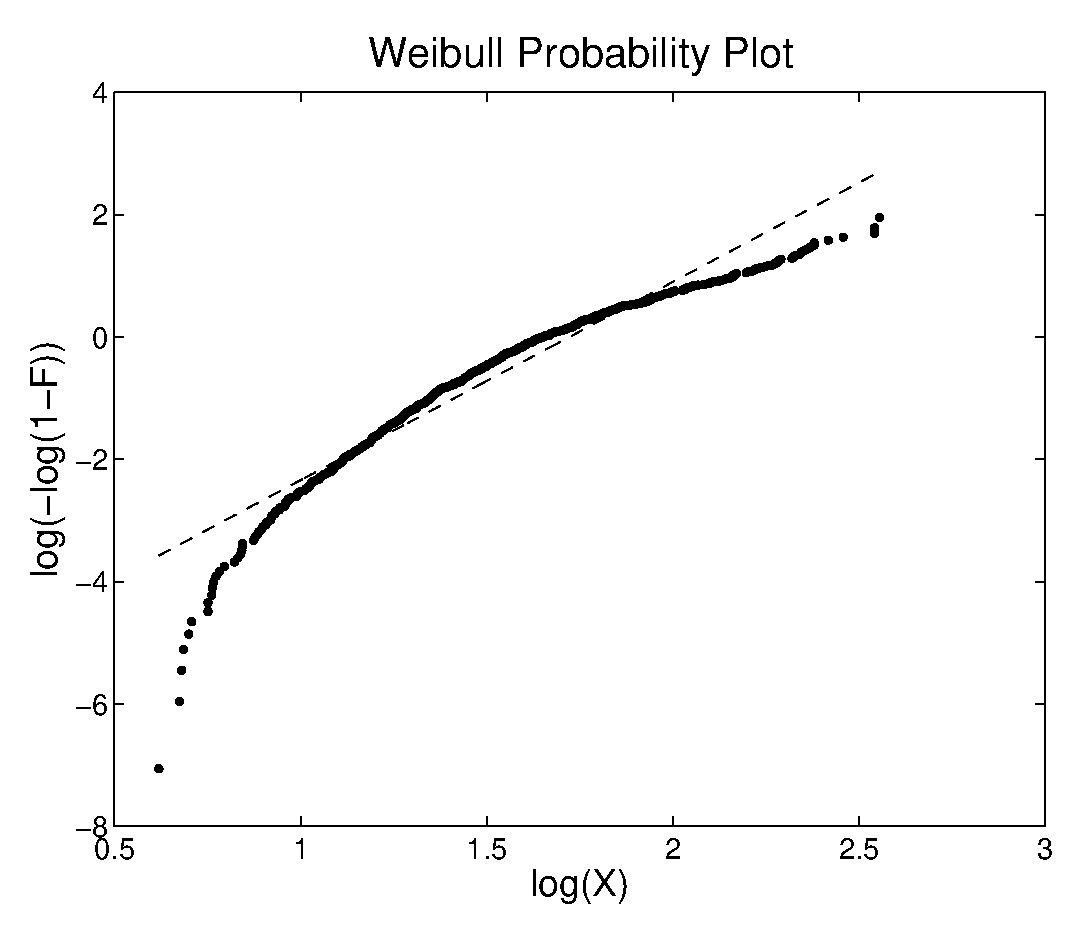
\includegraphics[height=55mm]{fig7-1a}
\end{minipage}}%
\hfill
\subfigure[]{%
\begin{minipage}[b]{0.48\textwidth}%
\centering 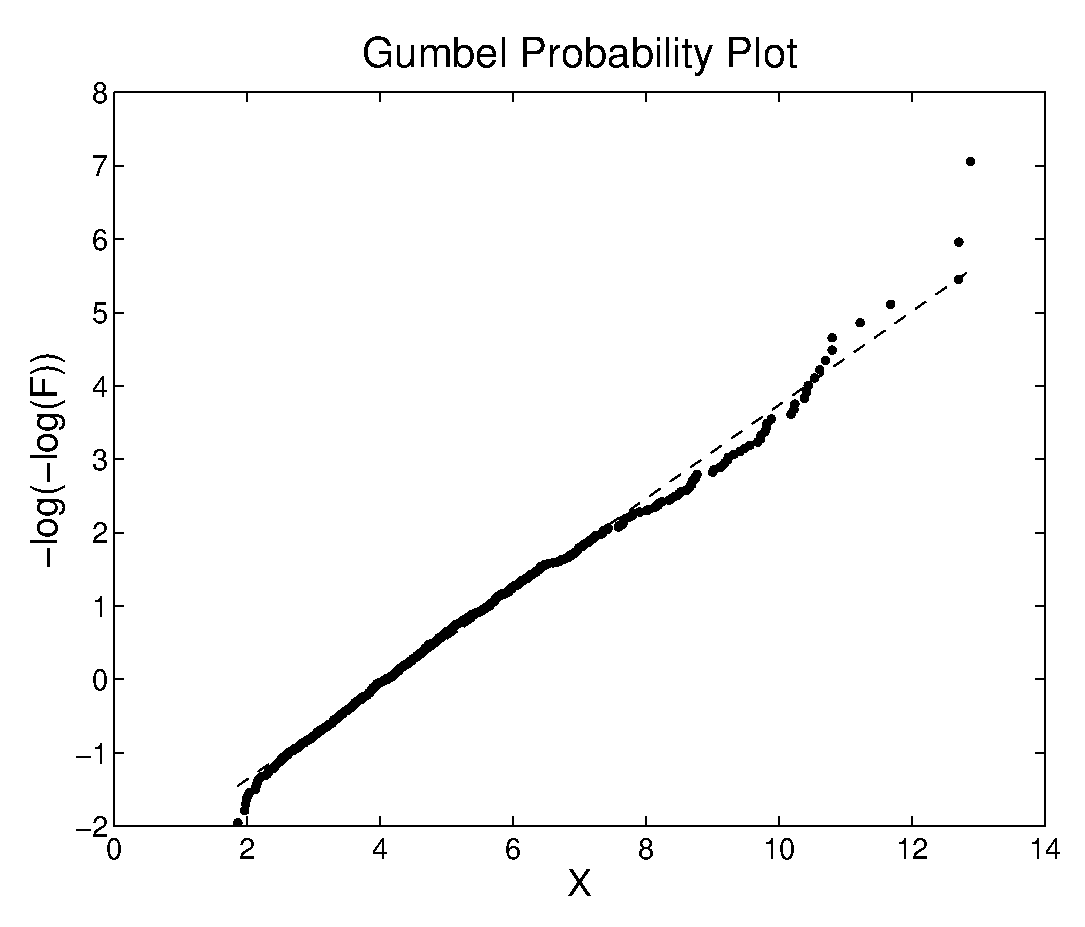
\includegraphics[height=55mm]{fig7-1b}
\end{minipage}}
\subfigure[]{%
\begin{minipage}[b]{0.48\textwidth}%
\centering 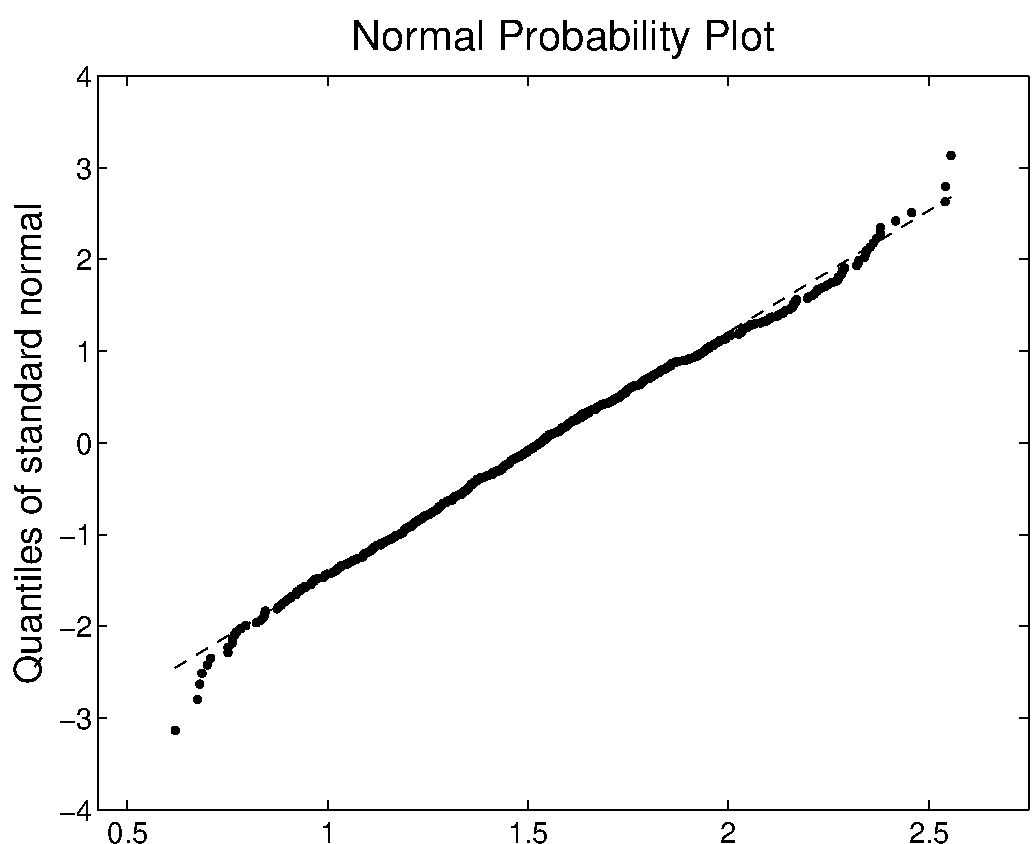
\includegraphics[height=55mm]{fig7-1c}
\end{minipage}}\hspace{5mm}
\subfigure[]{%
\begin{minipage}[b]{0.48\textwidth}%
\centering 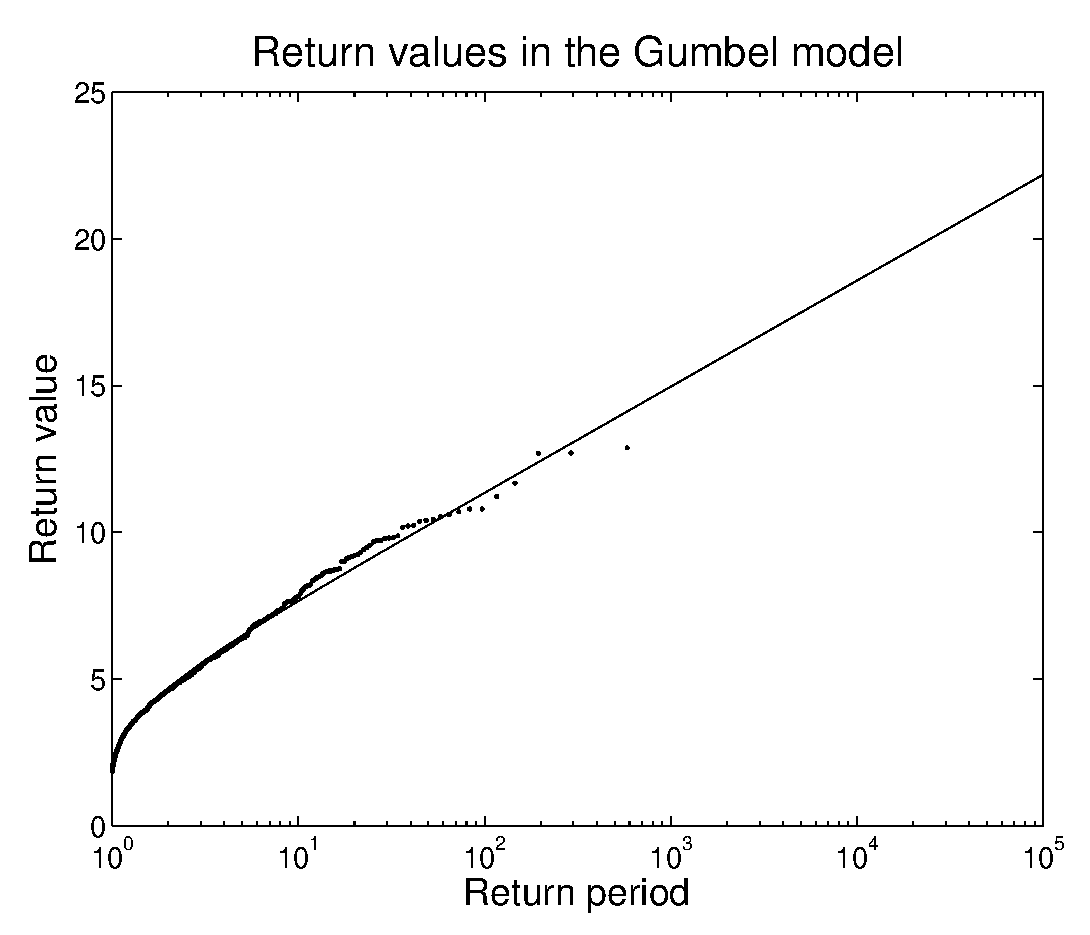
\includegraphics[height=55mm]{fig7-1d}
\end{minipage}}
  \caption[Significant wave-height data]{
Significant wave-height data: (a) on Weibull paper, (b) on
    Gumbel paper, (c) logarithm of data on Normal probability paper,
and (d) return values calculated in the Gumbel model with observed data.}
  \label{fig7-1}
\end{figure}

This will result in a two element vector {\tt wei = [ahat chat]} with
estimated values of the parameters $(a, c)$ in (\ref{eq:Wei}). The empirical
distribution function of the input data is plotted automatically in a
Weibull diagram with scales chosen to make the Weibull distribution function
equal to a straight line. The horizontal scale is logarithmic in the
observations $x$, and the vertical scale is linear in the {\em reduced
  variable} $\log (-\log (1 - F(x)))$;
see Figure~\ref{fig7-1}(a). Obviously, a Weibull distribution is
not very well suited to describe the significant wave-height data.

To illustrate the use of the Gumbel distribution we plot and estimate
the parameters $(a, b)$ in the Gumbel distribution (\ref{eq:Gum}) for the
data in {\tt Hs}. The command
{\small\begin{verbatim}
      gum = plotgumb(Hs)
\end{verbatim}}
\index[xcmds]{{\tt plotgumb}}\index[xentr]{Gumbel distribution!probability paper}
\noindent
results in a vector {\tt gum} with estimated values
{\tt [ahat bhat]} and the plot in Figure~\ref{fig7-1}(b). Here the
horizontal axis is linear in the observations $x$ and the vertical
axis carries the reduced variable $- \log (- \log(F(x)))$. The data
shows a much better fit to the Gumbel than to a Weibull
distribution.

A distribution that is often hard to distinguish from
the Gumbel distribution is the Lognormal distribution, and making a
Normal probability plot of the logarithm of {\tt Hs} in
Figure~\ref{fig7-1}(c) also shows a good fit.
{\small\begin{verbatim}
      plotnorm(log(Hs),1,0);
\end{verbatim}}
\index[xcmds]{{\tt plotnorm}}

The parameter estimation in {\tt plotgumb} and {\tt plotweib} is done
by fitting a straight line to the empirical distribution functions in
the diagrams and using the relations
\begin{equation}
  \log\{-\log[1-F_{W}(x;a,c)]\}=c\log(x)-c\log(a),
\end{equation}
and
\begin{equation}
  -\log\{-\log[F_{G}(x;a,b)]\}=x/a-b/a,
\end{equation}
to relate parameters to intercepts and slopes of the estimated lines.
In the following section we shall describe some more statistical
techniques for parameter estimation in the Generalized Extreme Value
distribution.

\subsection{Return value and return period }\label{subsec:returnvaluesWeibGumb}
The results of an extreme value analysis is often expressed in terms of
{\em return values} or {\em return levels},
which are simply related to the quantiles of the distribution.
A return value is always coupled to a {\em return period},
expressed in terms of the length of an observation period, or the
number of (independent) observations of a random variable.
\index[xentr]{return!level}\index[xentr]{return!period}

Suppose we are interested in the return levels for the largest significant
wave height that is observed during one year at a measuring site. Denote by
$M_{H_s}^k$ the maximum during year number $k$ and let its distribution
function be $F(x)$. Then the $N$-year return level, $s_{N}$, is defined by
\begin{equation}
F(s_{N}) = 1 - 1/N.
\label{eq:quantile}
\end{equation}
For example, $P(H_s > s_{100}) = 1 - F(s_{100}) = 1/100$, which means that,
\begin{itemize}\setlength\itemsep{-1mm}
\item
the probability that the level
$s_{100}$ is exceeded during one particular year is $0.01$,
\item
on the average, the yearly maximum significant wave height
exceeds $s_{100}$ one year in 100 years,
(note that there may be several exceedances
during that particular year),
\item
the probability that  $s_{100}$ is exceeded {\em at least} one
time during a time span of 100 years is $1-(1-0.01)^{100} \approx
1-1/e = 0.6321$,
provided years are independent.
\end{itemize}

To make it simple, we consider the Gumbel distribution, and
get, from (\ref{eq:quantile}), the $T$-year return value for the
yearly maximum in the Gumbel distribution (\ref{eq:Gum}):
\begin{equation}
s_T = b - a \log (- \log (1 - 1/T)) \approx b + a \log T,
\label{eq:GumbelreturnA}
\end{equation}
where the last approximation is valid for large $T$-values.

As an example we show a return value plot for the Atlantic data,
as if they represented a sequence of yearly maxima.
Figure~\ref{fig7-1}(d) gives the
return values as a function of the return period for the Atlantic data.
The \progname{-commands} are:
{\small
\begin{verbatim}
      T = 1:100000;
      sT = gum(2) - gum(1)*log(-log(1-1./T));
      semilogx(T,sT), hold on
      N = 1:length(Hs); Nmax = max(N);
      plot(Nmax./N,sort(Hs,'descend'),'.')
      title('Return values in the Gumbel model')
      xlabel('Return priod')
      ylabel('Return value'), hold off
\end{verbatim}
}

In the next section we shall see a more realistic example of return
value analysis. The Atlantic data did not represent yearly maxima and
the example was included only as an alternative way to present the result
of a Gumbel analysis.

\section{The GPD and GEV families}\label{sec:GPD_GEV}

The Generalized Pareto Distribution (GPD)
\index[xentr]{Generalized Pareto!characteristics}  has the distribution function
\begin{equation}
  \mbox{GPD:} \qquad
  F(x; k, {\sigma})  =
  \left\{
  \begin{array}{ll}
  1 - \left( 1 - kx/{\sigma}\right)^{1/k},
  & \quad \mbox{if $k \neq 0$},\\[0.5em]
  1 - \exp \{-x/{\sigma}\}, & \quad \mbox{if $k = 0$},
  \end{array}
  \right.
  \label{eq:GPD}
\end{equation}
for $0 < x < \infty$, if $k \leq 0$, and for $0 < x < {\sigma}/k$, if $k
> 0$. The Generalized Extreme Value distribution (GEV)
\index[xentr]{Generalized Extreme Value!characteristics}
has distribution function
\begin{equation}
  \mbox{GEV:} \qquad F(x; k, {\mu}, {\sigma})  =
  \left\{
  \begin{array}{ll}
  \exp \left\{ - (1 - k(x-{\mu})/{\sigma})^{1/k}\right\},
  & \quad \mbox{if $k \neq 0$},\\[0.5em]
  \exp \left\{ - \exp \{ - (x-{\mu})/{\sigma}\} \right\},
  & \quad \mbox{if $k = 0$},
  \end{array}
  \right. \label{eq:GEV}
\end{equation}
for $k(x - {\mu}) < {\sigma}, \, {\sigma} > 0, \, k, \, {\mu}$
arbitrary.
The case $k=0$ is interpreted as the limit when $k \to 0$ for both
distributions.

Note that the Gumbel distribution is a GEV distribution with $k=0$
and that the Weibull distribution is equal to a reversed GEV
distribution with $k=1/c$, ${\sigma} = a/c$, and  ${\mu} = -a$,
i.e.\ if $~W$ has a Weibull distribution with parameters $(a,
c)$ then $- W$ has a GEV distribution with $k=1/c$, ${\sigma}= a/c$,
and ${\mu} = -a$.

The estimation of parameters in the GPD and GEV distributions is not
a simple matter, and no general method exists, which has uniformly good
properties for all parameter combinations. \progname{} contains
algorithms for plotting of distributions and estimation of parameters
with four different methods, suitable in different regions.

\subsection{Generalized Extreme Value distribution}

For the Generalized Extreme Value (GEV) distribution the estimation
methods used in the \progname{} toolbox are
the Maximum Likelihood (ML) method and the
method with Probability
Weighted Moments (PWM),
described in \cite{PrescottAndWalden1980Maximum} and
\cite{HoskingEtal1985Estimation}. The
programs have been adapted to \ML{} from a package of S-Plus routines
described in \cite{Borg1992XS}.

We start with the significant wave-height data for the \verb+Atlantic+ data,
stored in {\tt Hs}. The command
{\small\begin{verbatim}
      gev = fitgev(Hs,'plotflag',2)
\end{verbatim}}
\index[xcmds]{{\tt fitgev}}
\index[xentr]{Generalized Extreme Value!distribution, GEV}
\index[xentr]{Generalized Extreme Value!parameter estimation}
\noindent
will give estimates {\tt gev.params = [khat sigmahat muhat]}
of the parameters $(k, {\sigma}, {\mu})$
in the GEV distribution~(\ref{eq:GEV}).
The output matrix field {\tt gev.covariance} will contain the
estimated covariance matrix of the estimates. The program also gives
a plot of the empirical distribution together with the
best fitted distribution and two diagnostic plots that give indications
of the goodness of fit; see Figure~\ref{fig7-2}.

 \begin{figure}
%\subfigure[]{%
%\begin{minipage}[b]{0.5\textwidth}%
%\centering \includegraphics[width=\defwidth]{fig7-2a}
%\end{minipage}}%
%\hfill
%\subfigure[]{%
%\begin{minipage}[b]{0.5\textwidth}%
%\centering \includegraphics[width=\defwidth]{fig7-2b}
%\end{minipage}}
\centerline{
  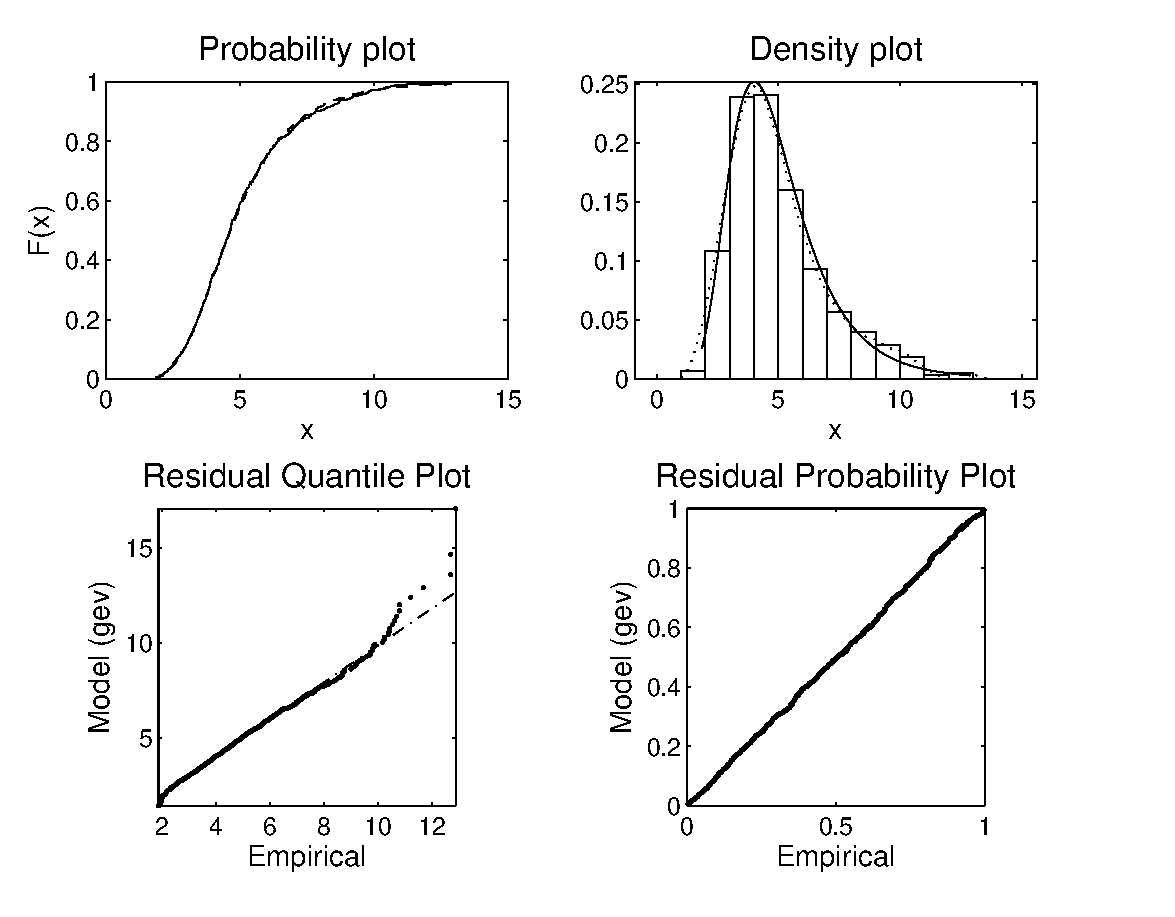
\includegraphics[width=\onefigwidth]{fig7-2ny}
}
\vspace{-3mm}
  \caption[Observed and estimated distribution
of significant wave-height]{
Empirical distribution (solid), cdf and pdf,
of significant wave-height in {\tt atlantic} data, with estimated (dashed)
  Generalized Extreme Value distribution, and two diagnostic plots og
goodness of fit.}
  \label{fig7-2}
\end{figure}

The routine \index[xcmds]{{\tt plotkde}}
{\tt plotkde}, which is a simplified version of the kernel density
estimation routines in {\tt kdetools}, is used to compare the GEV
density given estimated parameters with a non-parametric estimate
(note that {\tt plotkde} can be slow for large data sets like
{\tt Hs}).
The commands
{\small\begin{verbatim}
      clf
      x = linspace(0,14,200);
      plotkde(Hs,[x;pdfgev(x,gev)]')
\end{verbatim}}
\noindent
will give the upper right diagram in Figure~\ref{fig7-2}.

The default estimation algorithm for the GEV distribution is the
method with Probability Weighted Moments (PWM). An optional second
argument, {\tt fitgev(Hs, method)}, allows a choice between
the PWM-method (when {\tt method = 'pwm'}) and the alternative ML-method
(when {\tt method = 'ml'}). The variances of the ML estimates are
usually smaller than those of the PWM estimates. However, it is
recommended that one first uses the PWM method, since it works for a
wider range of parameter values.
\begin{figure}[tbh]
\centerline{
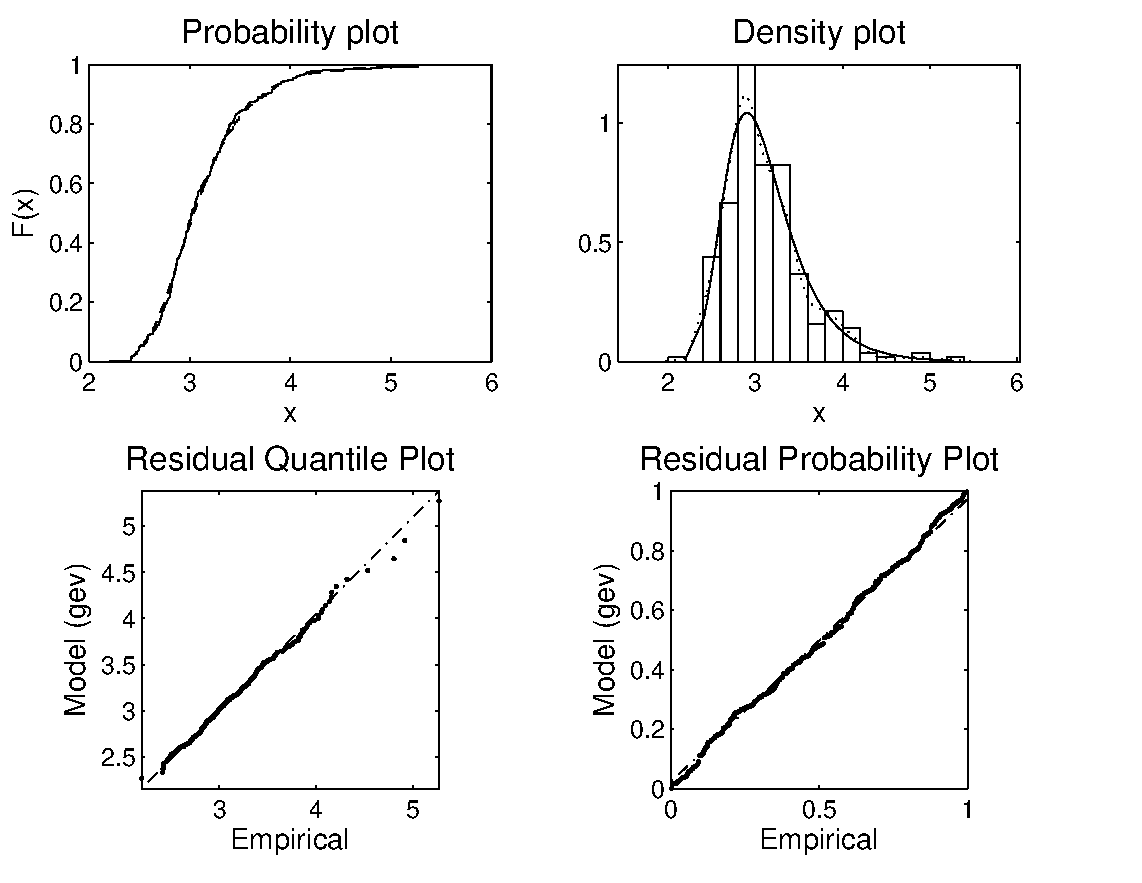
\includegraphics[width=\onefigwidth]{gevyura87}
}
\vspace{-3mm}
\caption[GEV analysis of sea level data]{
GEV analysis of 285 maxima over 5~minute intervals of sea level
data Yura87.}
\label{fig7-2b}
\end{figure}

\begin{rtex}{yura87}{Wave data from the Yura station}
The \progname{} toolbox contains a data set {\tt yura87} of more than 23~hours
of water level registrations at the Poseidon platform in the Japan Sea;
see {\tt help yura87}. Sampling rate is 1~Hz and to smooth data we
interpolate to 4~Hz, and then group the data into a matrix with 5~minutes
of data in each column, leaving out the last, unfinished period.
{\small
\begin{verbatim}
     xn = load('yura87.dat');
     XI = 0:0.25:length(xn);
     N  = length(XI); N = N-mod(N,4*60*5);
     YI = interp1(xn(:,1),xn(:,2),XI(1:N),'spline');
     YI = reshape(YI,4*60*5,N/(4*60*5)); % Each column holds
                            %  5 minutes of interpolated data.
\end{verbatim}
}
\noindent
It turns out that the mean value and standard deviation change slowly
during the measuring period, and we therefore standardize each column
to zero mean and unit variance, before we take the maximum over each
5~minute interval and perform the GEV analysis; compare the results
with those in the simpler analysis in Section~\ref{sec:extreme_example}.
{\small
\begin{verbatim}
     Y5 = (YI-ones(1200,1)*mean(YI))./(ones(1200,1)*std(YI));
     Y5M = max(Y5);
     Y5gev = fitgev(Y5M,'plotflag',2)
\end{verbatim}
}\index[xcmds]{{\tt fitgev}}
The estimated parameters in {\tt Y5gev.params} are $k = -0.314$ with a 95\%
confidence interval of $(-0.12, 0.06)$, indicating that a Gumbel
distribution might be an acceptable choice. Location and scale are estimated
to $\mu = 2.91$ and $\sigma = 0.34$. Figure~\ref{fig7-2b}
shows a good fit to the GEV model for the series of 5~minute
maxima in the (standardized) Yura series, except for the
few largest values, which are underestimated by the model.
This is possibly due to a few short periods
with very large variability in the data.
\end{rtex}

\subsection{Generalized Pareto distribution}

For the Generalized Pareto distribution (GPD) the \progname{} uses
the method with Probability Weighted Moments (PWM), described in
\cite{HoskingAndWallis1987Parameter}, and the standard Method of
Moments (MOM), as well as a
general method suggested by Pickands, in
\cite{Pickands1975Statistical}. S-Plus routines
for these methods are described in \cite{Borg1992XS}.

The GPD is often used for exceedances over high levels, and it is
well suited as a model for significant wave heights.
To fit a GPD to the exceedances in the {\tt atlantic}
$H_s$ series over of thresholds 3 and 7, one uses the commands
{\small\begin{verbatim}
      gpd3 = fitgenpar(Hs(Hs>3)-3,'plotflag',1);
      figure
      gpd7 = fitgenpar(Hs(Hs>7),'fixpar',...
                   [nan,nan,7],'plotflag',1);
\end{verbatim}}
\index[xcmds]{{\tt fitgenpar}}
\index[xentr]{Generalized Pareto!parameter estimation}
\index[xentr]{Generalized Pareto!distribution, GPD}
\noindent
This will give estimates {\tt gpd.params = [khat sigmahat]} of the parameters $(k,
{\sigma})$ in the Generalized Pareto distribution~(\ref{eq:GPD}) based on
exceedance data
{\tt Hs(Hs>u)-u}. The optional output matrix {\tt gpd.covariance} will contain the
estimated covariance matrix of the estimates.
The program also gives a plot of the empirical
distribution together with the best fitted distribution; see
Figure~\ref{fig7-3}. The fit is better for exceedances over level
7 than over 3, but there are less data available, and the confidence bounds are wider.

\begin{figure}
\subfigure[]{%
\begin{minipage}[b]{0.5\textwidth}%
\centering 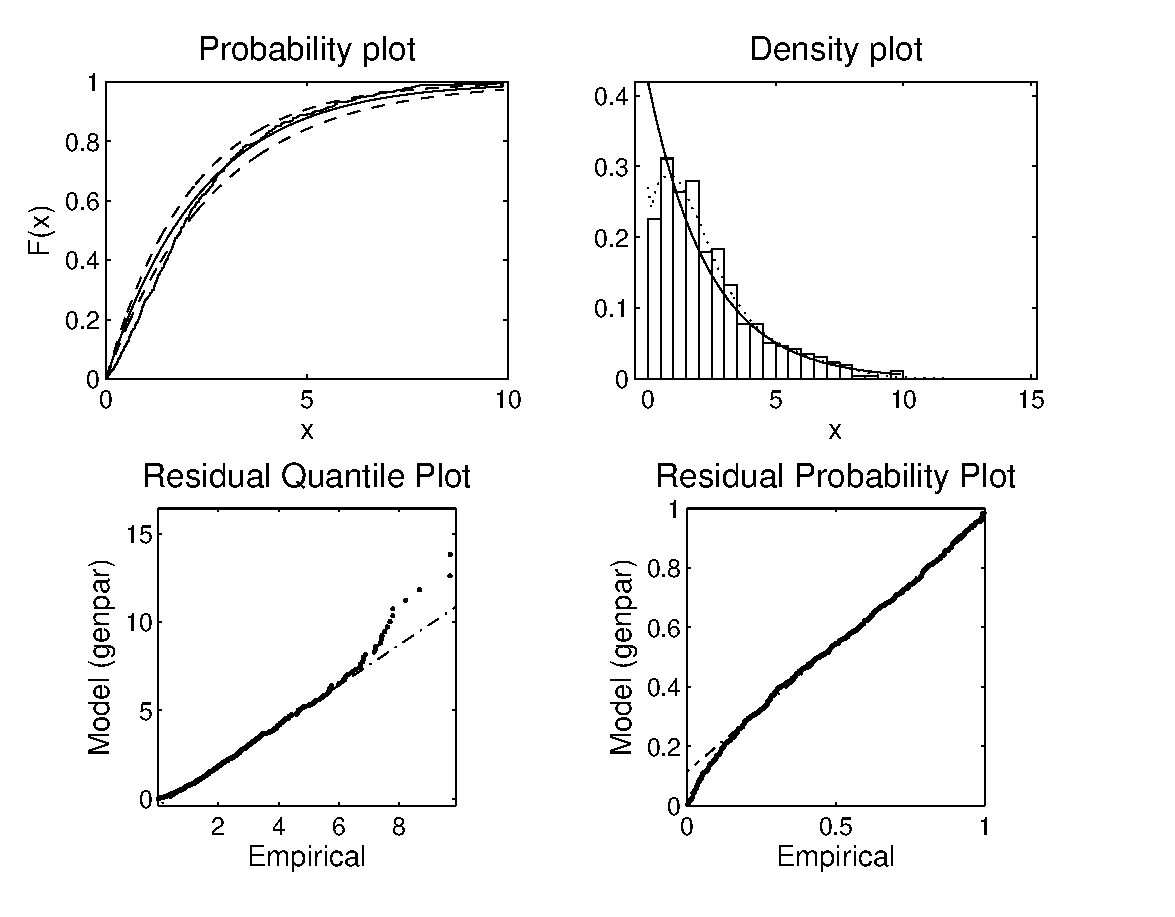
\includegraphics[width=75mm]{fig7-3a}
\end{minipage}}%
\hfill
\subfigure[]{%
\begin{minipage}[b]{0.5\textwidth}%
\centering 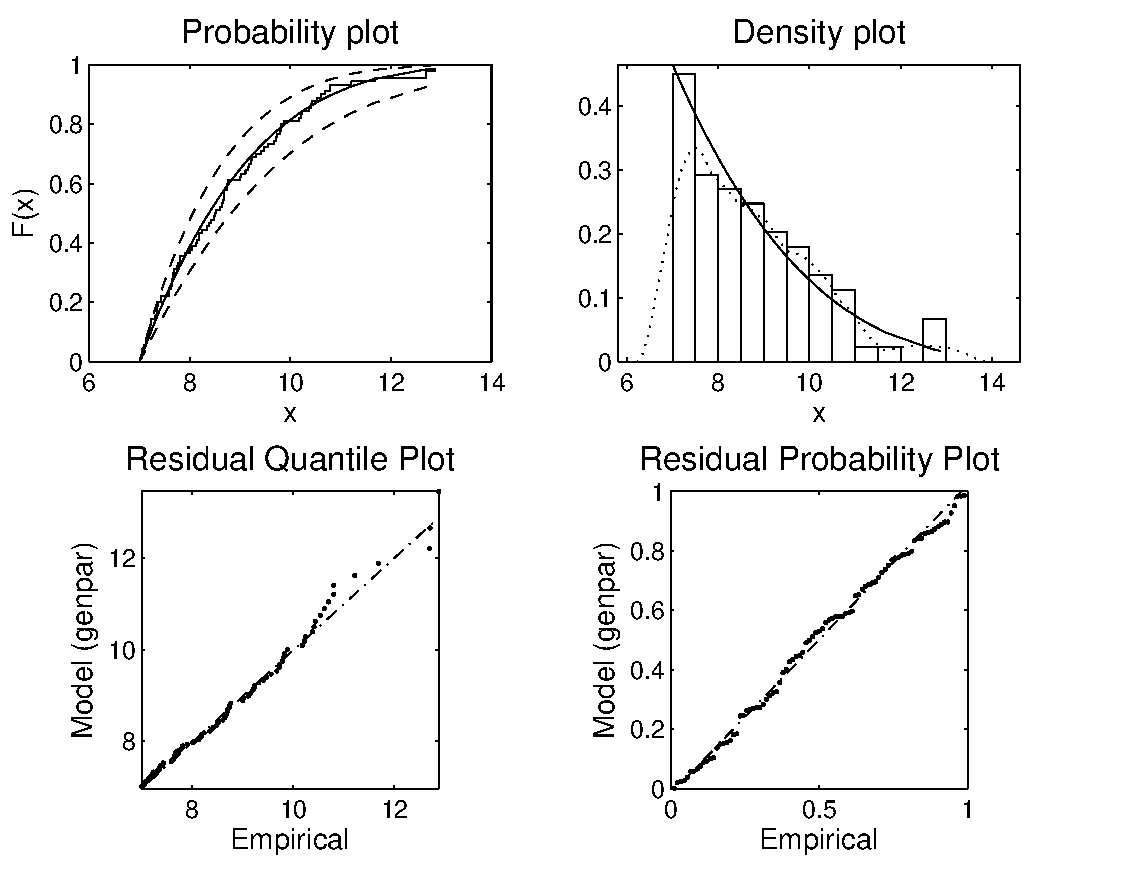
\includegraphics[width=75mm]{fig7-3b}
\end{minipage}}
\vspace{-4mm}
  \caption[Exceedances of significant wave-height data over levels]
{(a) Exceedances of significant wave-height data over level 3,
  (b) Significant wave-heigh over level 7, in {\tt atlantic} data}
  \label{fig7-3}
\end{figure}

The choice of estimation method is rather dependent on the
actual parameter values.  The default estimation algorithm in
\progname{} for
estimation in the Generalized Pareto distribution is the Maximum
Product of Spacings (MPS) estimator  since it works for all
values of the shape \index[xentr]{maximum product of spacings (MPS)}
  parameter and have the same asymptotic properties as the Maximum
  Likelihood (ML) method  (when it is valid).
The Pickands' (PKD) and Least Squares (LS) estimator also work for
any value of the shape parameter $k$ in Eq.~(\ref{eq:GPD}).
   The ML method is only useful when $k \leq 1$, the PWM when $k>-0.5$,
  the MOM when $k>-0.25$. The variances of the ML estimates are usually
  smaller than those of the other estimators. However, for small sample
  sizes it is recommended to use the PWM, MOM or MPS if they are
  valid.

It is possible to simulate independent GEV and GPD observations in
\progname{}. The command series
{\small\begin{verbatim}
      Rgev = rndgev(0.3,1,2,1,100);
      gp = fitgev(Rgev,'method','pwm');
      gm = fitgev(Rgev,'method','ml','start',gp.params,...
                  'plotflag',0);
      x=sort(Rgev);
      plotedf(Rgev,gp,{'-','r-'}); hold on
      plot(x,cdfgev(x,gm),'--'); hold off
\end{verbatim}}
\index[xcmds]{{\tt rndgev}}
  \index[xcmds]{{\tt cdfgev}}\index[xcmds]{{\tt plotedf}}
\noindent
simulates 100 values from the GEV distribution with parameters
$(0.3,1,2)$, then estimates the parameters using two different methods
and plots the estimated distribution functions together with the
empirical distribution. Similarly for the GPD distribution.
{\small\begin{verbatim}
      Rgpd = rndgenpar(0.4,1,0,1,100);
      plotedf(Rgpd); hold on
      gp = fitgenpar(Rgpd,'method','pkd','plotflag',0);
      x=sort(Rgpd);
      plot(x,cdfgenpar(x,gp))
      gw = fitgenpar(Rgpd,'method','pwm','plotflag',0);
      plot(x,cdfgenpar(x,gw),'g:')
      gml = fitgenpar(Rgpd,'method','ml','plotflag',0);
      plot(x,cdfgenpar(x,gml),'--')
      gmps = fitgenpar(Rgpd,'method','mps','plotflag',0);
      plot(x,cdfgenpar(x,gmps),'r-.'); hold off
\end{verbatim}}
\index[xcmds]{{\tt rndgenpar}}\index[xcmds]{{\tt cdfgenpar}}
\noindent
with four different methods of parameter estimation.
The results are shown in Figure~\ref{fig7-4}(a) and (b).

\begin{figure}
\subfigure[]{%
\begin{minipage}[b]{0.5\textwidth}%
\centering 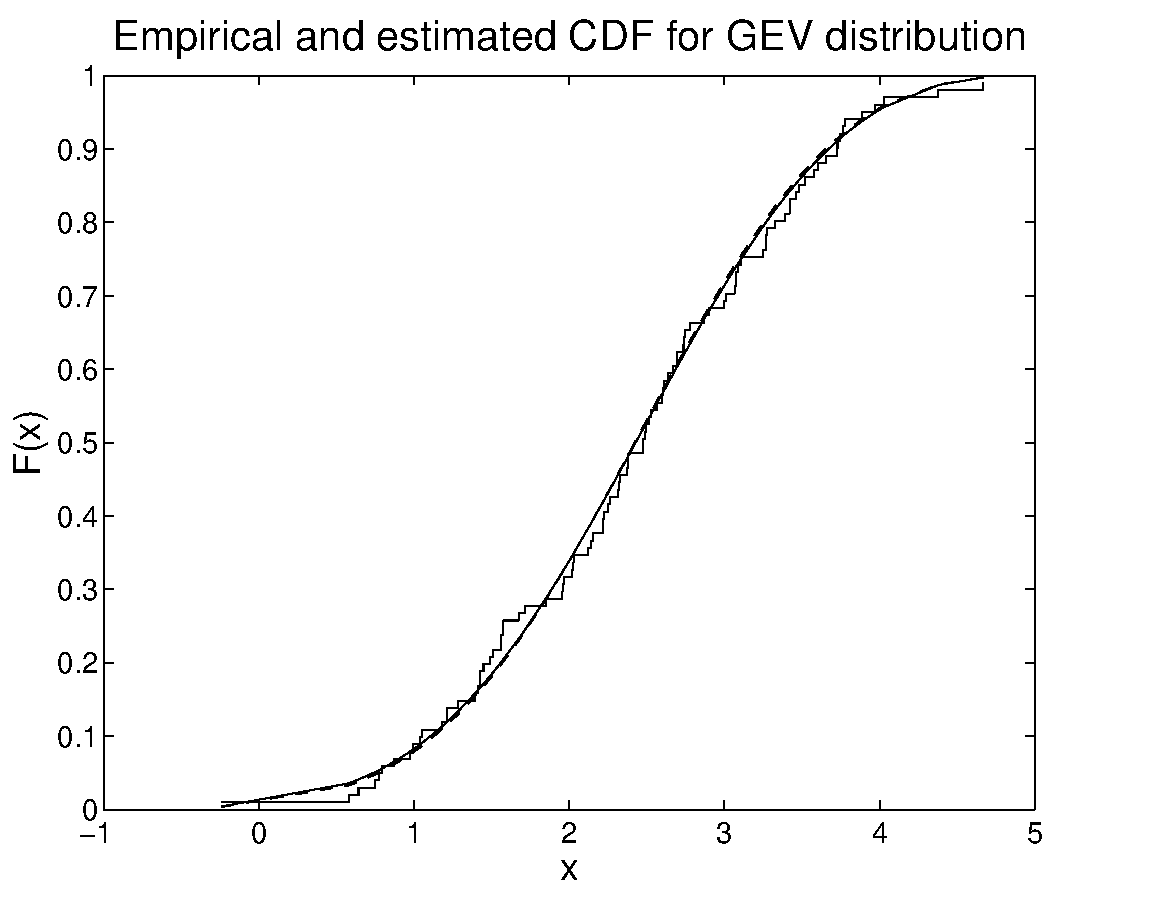
\includegraphics[width=\defwidth]{fig7-4a}
\end{minipage}}%
\hfill
\subfigure[]{%
\begin{minipage}[b]{0.5\textwidth}%
\centering 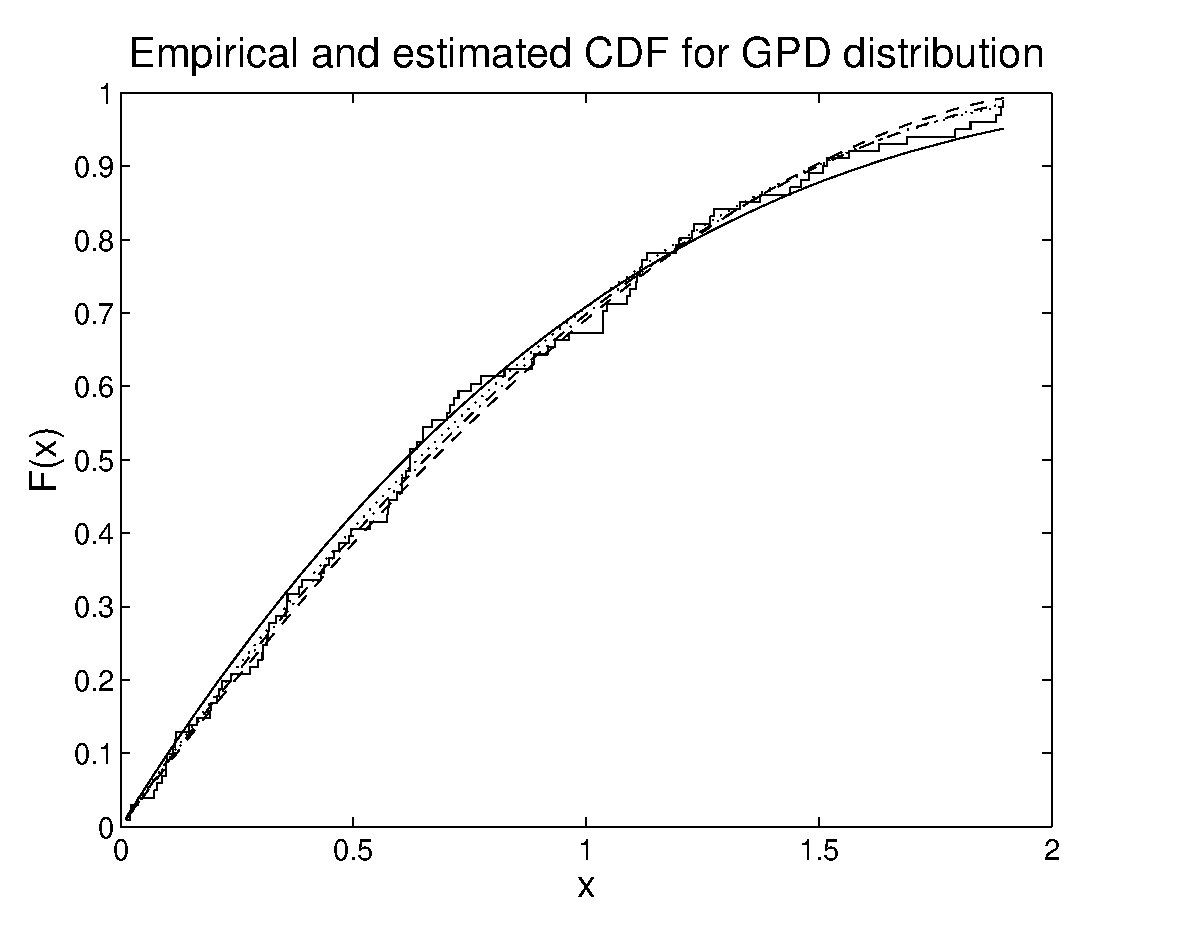
\includegraphics[width=\defwidth]{fig7-4b}
\end{minipage}}
\vspace{-4mm}
  \caption[Empirical and estimated distribution functions for GEV variables]
{Empirical (solid) distributions and estimated (dashed) distribution functions
  for 100~observations of GEV (a) and GPD (b) variables.}
  \label{fig7-4}
\end{figure}

%\progname{} also contains random number generators from a broad variety
%of distributions; see {\tt help Contents} and
%Section~\ref{sec:extremevaluestatistics}.

\subsection{Return value analysis}\label{subsec_returnvalueanalysis}
As in the Gumbel model, one can calculate the return levels in the GEV
by inverting (\ref{eq:quantile}) with the GEV distribution function
(\ref{eq:GEV}). The return level corresponding to return period $N$
satisfies $1-F(s_N)=1/N$, so when $F$ is a GEV distribution function
with shape parameter $k \neq 0$,
\index[xentr]{return!level}\index[xentr]{return!period}
\begin{equation}
s_N = \mu + \frac{\sigma}{k} \left( 1 - (- \log (1 - 1/N) )^{k} \right)
\approx \mu + \frac{\sigma}{k} \left( 1 - N^{-k} \right),
\label{eq:return_gev}
\end{equation}
where the last expression holds for $N$ large, so one
can use $- \log (1 - 1/N) \approx 1/N$. As always in practice, the
parameters in the return level have to be replaced by their
estimated values, which introduces uncertainties in the computed
level.
\begin{cex}{yura87}
Applied to the {\tt yura87} data and the estimated GEV-model,
we perform the return level extrapolation by the commands,
{\small
\begin{verbatim}
      T = 1:100000;
      k = Y5gev.params(1); mu=Y5gev.params(3);
      sigma = Y5gev.params(2);
      sT = mu + sigma/k*(1-(log(1-1./T))^k);
      semilogx(T,sT), hold
      N = 1:length(Y5M); Nmax=max(N);
      plot(Nmax./N,sort(Y5M,'descend'),'.')
      title('Return values in the GEV model')
      xlabel('Return priod')
      ylabel('Return value')
      grid on; hold off
\end{verbatim}
}
\noindent
The result is shown in Figure~\ref{fig_yurareturn},
 consistent with the
quantile plot in Figure~\ref{fig7-2b}.
\end{cex}
\begin{figure}[tbh]
\centerline{
%\includegraphics[width=\defwidth]{yurareturn}
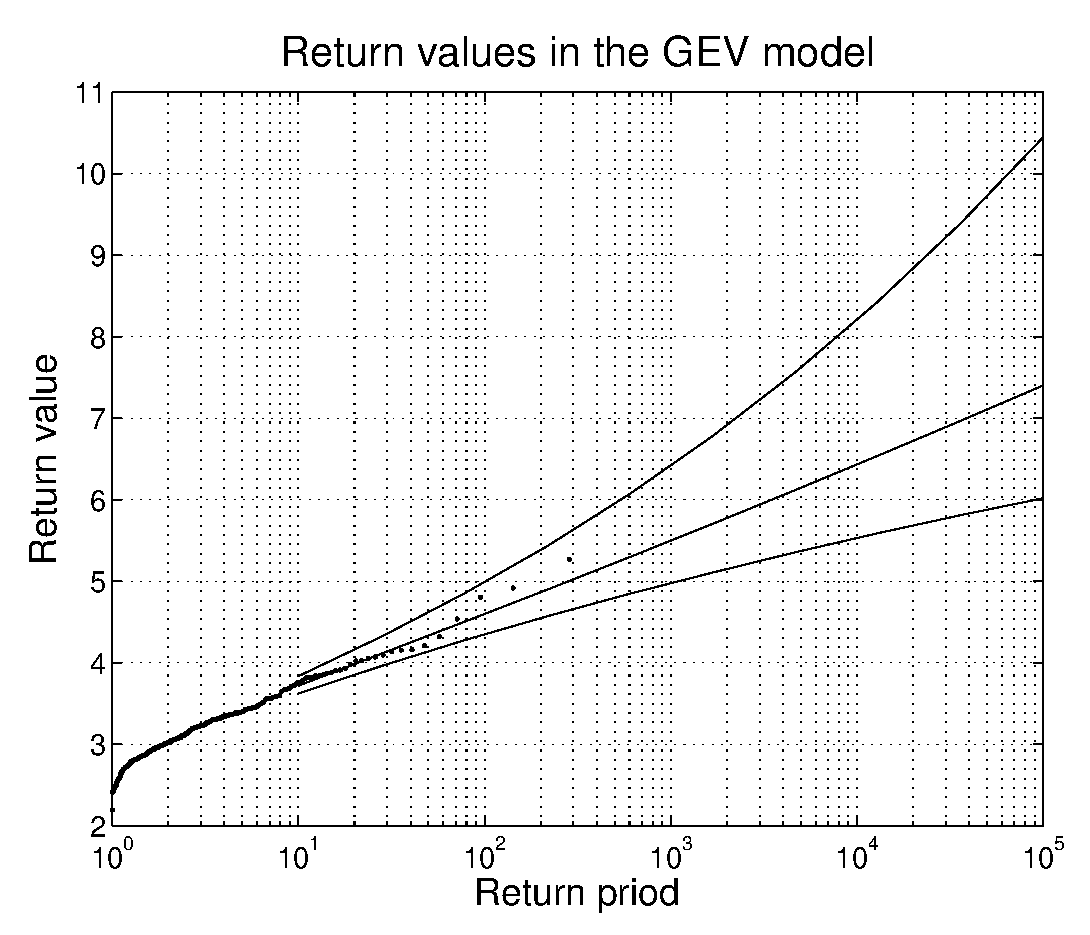
\includegraphics[width=\defwidth]{fig5_6}
}
\vspace{-3mm}
\caption[Return level extrapolation]{
Return level extrapolation in  {\tt yura87} data depends
on the good fit in the main part of the distribution. A few deviating
large observations are disturbing.}
\label{fig_yurareturn}
\end{figure}

\section{POT-analysis}

Peaks Over Threshold analysis (POT)
\index[xentr]{Peaks Over Threshold analysis, POT|(} is a systematic way to analyse
the distribution of the exceedances over high levels in order to
estimate extreme quantiles outside the range of observed values. The
method is based on the observation that the extreme tail of a
distribution often has a rather simple and standardized
form, regardless of the shape of the more central parts of the
distribution. One then fits such a simple distribution only to those
observations that exceed some suitable level, with the hope that
this fitted distribution gives an accurate fit to the
real distribution also in the more extreme parts. The level should be
chosen high enough for the tail to have approximately the
standardized form, but not so high that there remains too few
observations above it. After fitting a tail distribution one
estimates the distribution of the (random) number of exceedances over
the level, and then combines the tail distribution of the individual
exceedances with the distribution for the number of exceedances to
find the total tail distribution.

\subsection{Expected exceedance}\index[xentr]{Expected exceedance}
The simplest distribution to fit to the exceedances over a level $u$
is the Generalized Pareto distribution, GPD, with distribution function
(\ref{eq:GPD}).
Note that if a random variable $X$ follows a Generalized Pareto
distribution $F(x; k, {\sigma})$, then the exceedances over a level
$u$ is also GPD with distribution function
$F(x; k, {\sigma}-ku)$, with the same
$k$-parameter but with different (if $k \neq 0$)
scale parameter ${\sigma} - ku$,
$$
\pr (X > u + y \mid X > u) = \frac{
\left(1 - k \frac{u+y}{{\sigma}}\right)^{1/k}}
{\left(1 - k \frac{u}{{\sigma}}\right)^{1/k}}
= \left(1 - k \frac{y}{{\sigma}-ku}\right)^{1/k}.
$$

Another important property of the Generalized Pareto Distribution is
that if $k > -1$, then the mean exceedance over a level $u$ is a
linear function of $u$:
$$
\ex (X -u  \mid X > u) = \frac{{\sigma} - ku}{1+k}.
$$
Plotting the mean exceedance as a function of $u$ can help on decide on
a proper threshold value. The resulting plot is called
\emph{Mean residual life plot}, also referred to as mean
excess plots in statistical literature.
The following command illustrate this for the significant
wave height {\tt atlantic} data: \index[xentr]{Mean residual life}
{\small\begin{verbatim}
      plotreslife(Hs,'umin',2,'umax',10,'Nu',200);
\end{verbatim}} \index[xcmds]{{\tt plotreslife}}
\noindent
The result is plotted in Figure~\ref{fig7-5}, and it seems to
exhibit an almost linear relationship for $u\geq 7$.

\begin{figure}
  \centering
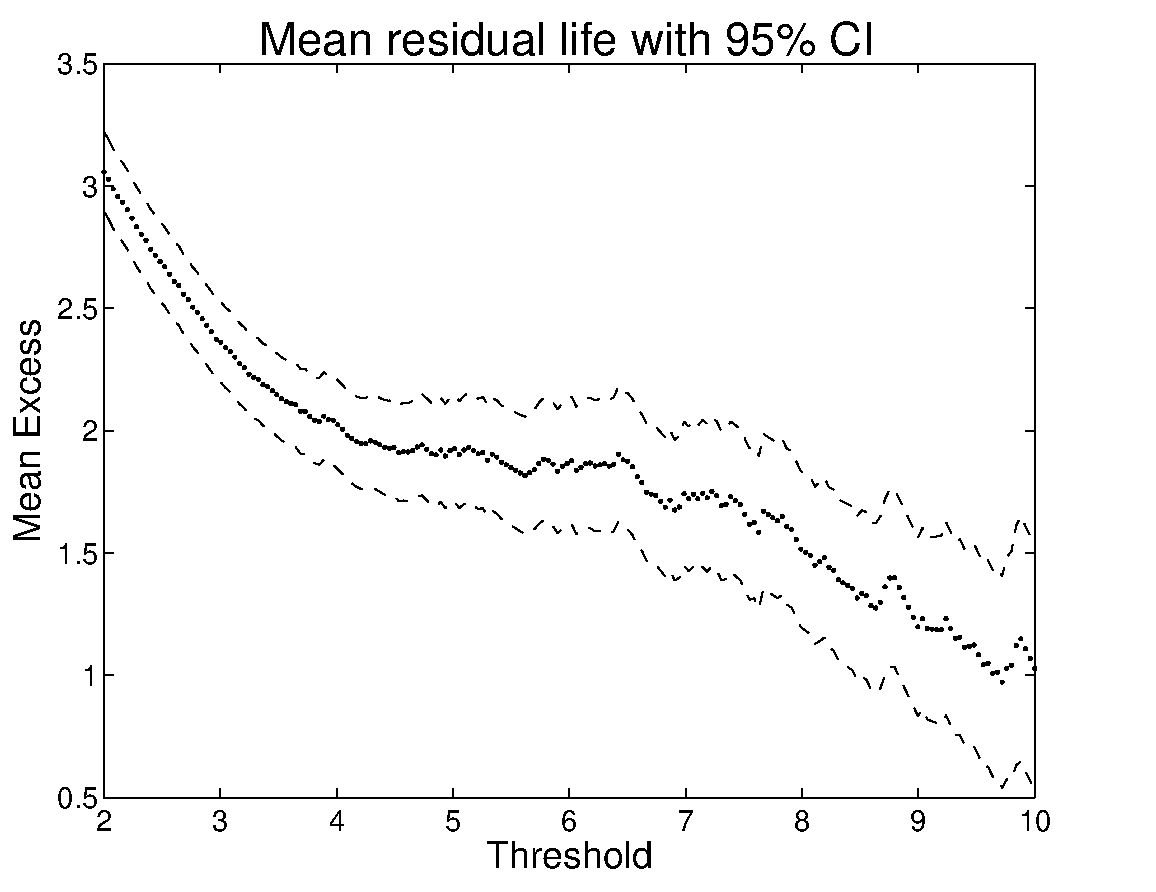
\includegraphics[width=\defwidth]{fig7-5}
\vspace{-3mm}
  \caption[Estimated expected exceedance over level $u$]
{Expected exceedance over level $u$ of  {\tt atlantic} data
as function of $u$.}
  \label{fig7-5}
\end{figure}

\subsection{Poisson + GPD = GEV}
If one is successful in fitting a Generalized Pareto distribution to the
tail of data, one would like to use the GPD to predict how
extreme values might occur over a certain period of time. One could, 
for example, want to predict the most extreme wave height that will appear
 during a year. If the distribution of the individual significant wave
height exceedances is GPD one can easily find e.g., the
distribution of the largest value of a fixed number of exceedances.
However, the number of exceedances is not fixed but random, and
then one has to combine the distribution of the random size of
individual exceedances with the random number of exceedances $N$,
before
one can say anything about the total maximum. If the level
$u$ is high we can, due to the Poisson approximation of the Binomial
distribution and neglecting the dependence of nearby values, assume
$N$ to have an approximate Poisson distribution.

Now there is a nice relationship between the Generalized Pareto
distribution and the Generalized Extreme Value distribution in this
respect: {\it the maximum of a Poisson distributed number of independent
GPD variables has a GEV distribution}. This follows by simple
summation of probabilities: if $N$ is a Poisson distributed
random variable with mean ${\mu}$, and $M_{N} = \max (X_1, X_2,
\ldots, X_{N})$ is the maximum of $N$ independent GPD variables
then,
\begin{eqnarray*}
  \pr (M_{N} \leq x) & = & \sum_{n=0}^{\infty} \pr (N = n) \cdot
  \pr (X_1 \leq x, X_2 \leq x, \ldots, X_n \leq x) \\
  & = & \sum_{n=0}^{\infty} e^{-{\mu}} \frac{{\mu}^n}{n!} \cdot
  \left( 1 - ( 1- k \frac{x}{{\sigma}})^{1/k}\right)^n \\
  & = & \exp \left\{- (1 - k(x-a)/b)^{1/k} \right\},
\end{eqnarray*}
which is the Generalized Extreme Value distribution with
$b={\sigma}/{\mu}^k$ and $a={\sigma}(1 - {\mu}^{-k})/k$.

This means that we can estimate the distribution of
the maximum significant wave
height during a winter (December -- February) months  from our data
set ${\tt Hs}$ by fitting a GPD to the exceedances over some level
$u$, estimating ${\mu}$ by the number of exceedances $N$ divided by
the number of months ($7\times 3\times
2=42$) and use the
above relation to fit a GEV distribution:
{\small\begin{verbatim}
      gpd7 = fitgenpar(Hs(Hs>7)-7,'method','pwm','plotflag',0);
      khat = gpd7.params(1);
      sigmahat = gpd7.params(2);
      muhat = length(Hs(Hs>7))/(7*3*2);
      bhat = sigmahat/muhat^khat;
      ahat = 7-(bhat-sigmahat)/khat;
      x = linspace(5,15,200);
      plot(x,cdfgev(x,khat,bhat,ahat))
\end{verbatim}} \index[xcmds]{{\tt cdfgev}}
\noindent
We have here used the threshold $u=7$ since the exceedances over this
level seem to fit well to a GPD distribution in Figures~\ref{fig7-3}(b)
and \ref{fig7-5}. A larger value will
improve the Poisson approximation to the number of exceedances but
give us less data to estimate the parameters.

Since we have approximately 14 data points for 41 complete months,
we can compute the monthly maxima {\tt mm} and fit a GEV distribution directly:
{\small\begin{verbatim}
      mm = zeros(1,41);
      for i=1:41                    % Last month is not complete
        mm(i) = max(Hs(((i-1)*14+1):i*14));
      end
      gev = fitgev(mm);
      plotedf(mm), hold on
      plot(x,cdfgev(x,gev),'--'), hold off
\end{verbatim}}

The results of the two methods agree very well in this case
as can be seen in Figure~\ref{fig7-6}, where the estimated
distributions are plotted
together with the empirical distribution of {\tt mm}.

\begin{figure}
  \centering
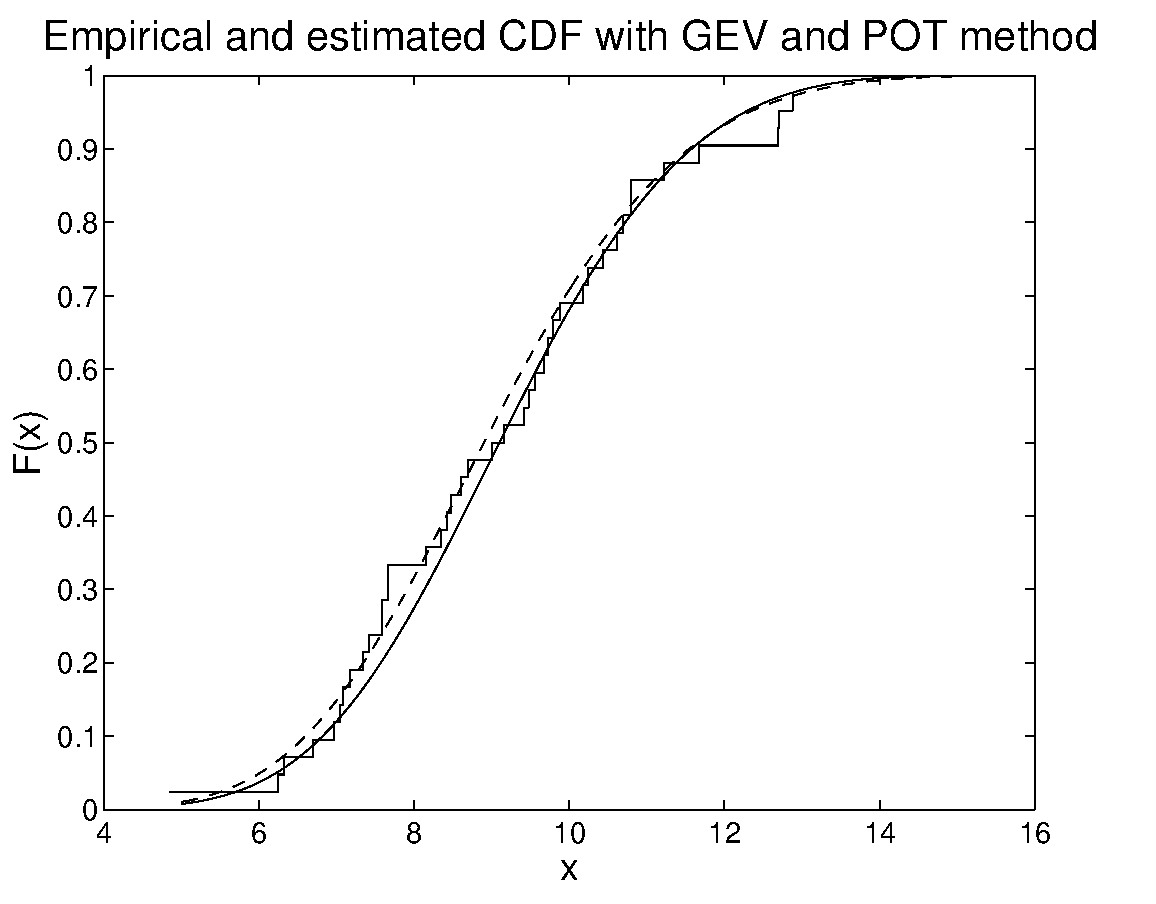
\includegraphics[width=\defwidth]{fig7-6}
\vspace{-3mm}
  \caption[Distribution functions of monthly maxima]
{Estimated distribution functions of monthly maxima with the
    POT method (solid), fitting a GEV (dashed) and the empirical distribution.}
  \label{fig7-6}
\end{figure}

\subsection{Declustering}\index[xentr]{Declustering}
The POT method relies on two properties of peaks over the selected
threshold: they should occur randomly in time according to an approximate
Poisson process, and the exceedances should have an approximate
GPD distribution and be approximately independent.
In practice, one does not always find a Poisson distribution for the
number of exceedances. Since extreme values sometimes have a tendency
to cluster, some declustering algorithm could be applied to identify
the largest value in each of the clusters, and then use a Poisson
distribution for the number of clusters. The selected peaks should be
sufficiently far apart for the exceedances to be independent.
The \progname{} toolbox
contains the routine {\tt decluster} to perform the declustering.
\index[xcmds]{{\tt decluster}}

To select the clusters and
check the Poisson character one can use the {\it dispersion index},
\index[xentr]{dispersion index} which is the ratio between
the variance and the expectation of the number of peaks. For a Poisson
distribution this ratio is equal to one. An acceptable peak separation
should give a dispersion index near one.

\begin{rtex}{decluster}{Declustering sea data}
We will extract peaks over threshold in the {\tt sea.dat}, which is
a recording of almost 40 minutes of sea level data, sampled at a rate
of {\tt 4[Hz]}.

We first define some parameters, {\tt Nmin,Tmin,Tb}, to control
the declustering, and to identify the peaks that exceed 90\% of
the median peak size and are separated by at least {\tt Tmin}.
{\small\begin{verbatim}
      Nmin = 7;                           % minimum number of extremes
      Tmin = 5;                           % minimum dist between extremes
      Tb = 15;                            % block period
      xx = load('sea.dat');
      timeSpan = (xx(end,1)-xx(1,1))/60;  % in minutes
      dt = xx(2,1)-xx(1,1);               % in seconds
      tc = dat2tc(xx);
      umin = median(tc(tc(:,2)>0,2));
      Ie0 = findpot(tc, 0.9*umin, Tmin);
      Ev = sort(tc(Ie0,2));
      Ne = numel(Ev)
      if Ne>Nmin && Ev(Ne-Nmin)>umin, umax = Ev(Ne-Nmin);
      else umax = umin;
      end
\end{verbatim}} \index[xcmds]{{\tt findpot}}
Next, we calculate the expected residual life and the
dispersion index for thresholds between
{\tt umin} and {\tt umax} and select an interval which is
compatible with the Poisson distribution for the number of peaks.

\begin{figure}
\subfigure[]{%
\begin{minipage}[b]{0.5\textwidth}%
\centering 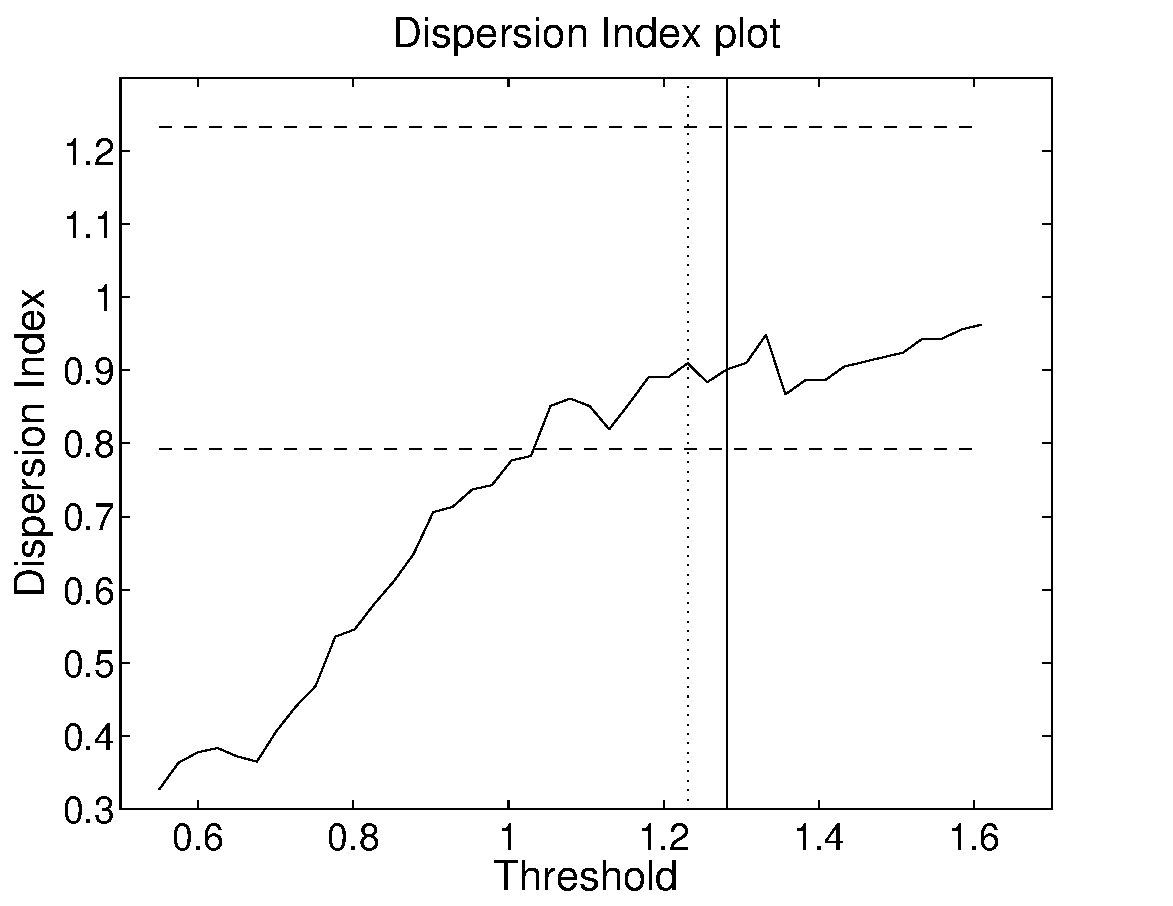
\includegraphics[height=60mm]{fig_decluster1b}
\end{minipage}}%
\hfill
\subfigure[]{%
\begin{minipage}[b]{0.5\textwidth}%
\centering 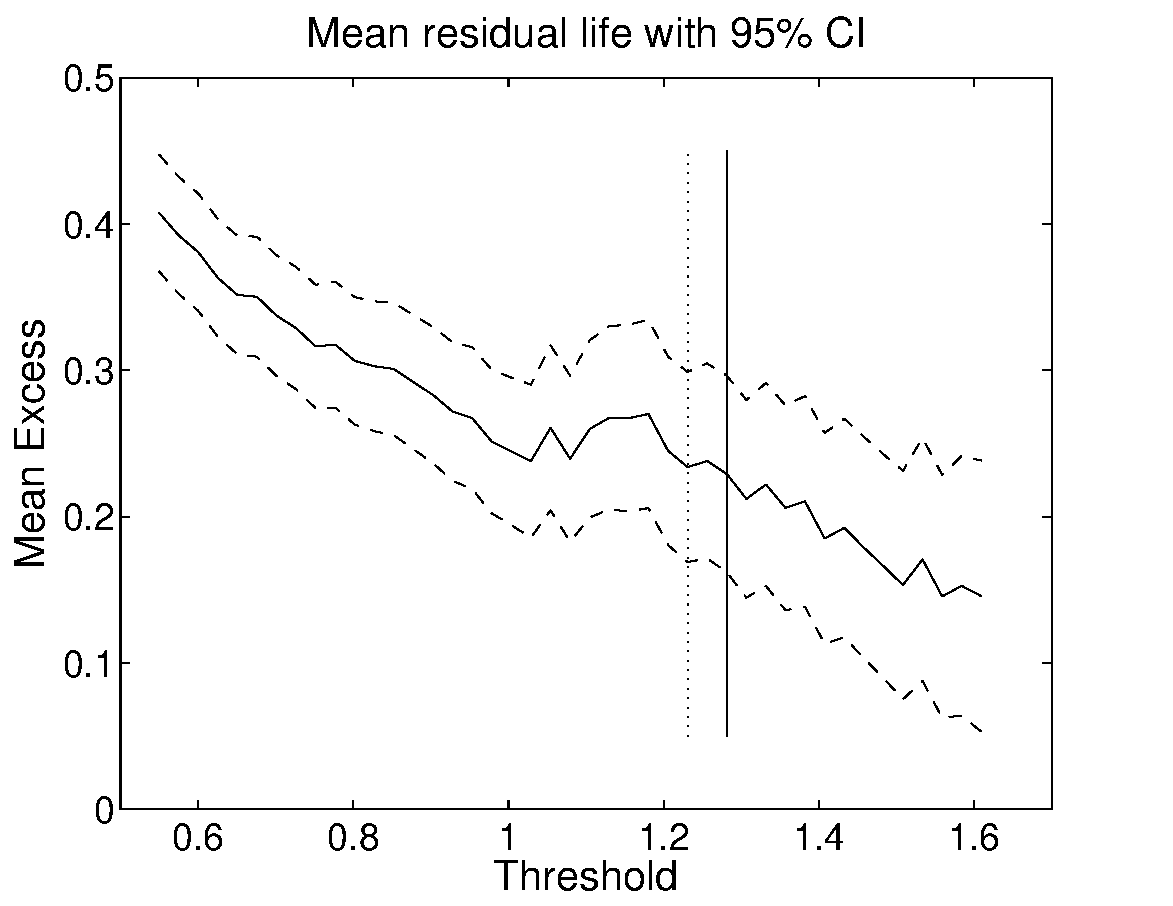
\includegraphics[height=60mm]{fig_decluster2b}
\end{minipage}}
\vspace{-3mm}
\caption[Threshold selection in POT analysis]{Threshold selection
in POT analysis. Dashed vertical line indicates threshold selected by the
dispersion index, solid line by the residual life analysis.}
\label{fig:thresholds}
\end{figure}

{\small\begin{verbatim}
      Nu = floor((umax-umin)/0.025)+1;
      u = linspace(umin,umax,Nu);
      mrl = reslife(Ev, 'u',u);
      umin0 = umin;
      for io = numel(mrl.data):-1:1,
        CI = mrl.dataCI(io:end,:);
        if ~(max(CI(:,1))<=mrl.data(io) && mrl.data(io)<=min(CI(:,2))),
            umin0 = mrl.args(io); break;
        end
      end
      [di, threshold, ok_u] = ...
            disprsnidx(tc(Ie0,:), 'Tb', Tb, 'alpha',0.05, 'u',u);
\end{verbatim}} \index[xcmds]{{\tt reslife}}
The plots from the following commands are shown in Figure~\ref{fig:thresholds}.
It seems as if {\tt threshold = 1.23[m]} is a suitable threshold.
{\small\begin{verbatim}
      figure(1); plot(di)
      vline(threshold)      % Threshold from dispersion index
      vline(umin0,'g')      % Threshold from mean residual life plot
      figure(2); plot(mrl)
      vline(threshold)      % Threshold from dispersion index
      vline(umin0,'g')      % Threshold from mean residual life plot
\end{verbatim}}
A GPD fit for peaks above {\tt 1.23[m]} with diagnostic
plot is obtained by the  commands
{\small\begin{verbatim}
      Ie = findpot(tc, threshold, Tmin);
      lambda = numel(Ie)/timeSpan; % # Y>threshold per minute
      varLambda = lambda*(1-(dt/60)*lambda)/timeSpan;
      stdLambd = sqrt(varLambda)
      Ev = tc(Ie,2);
      phat = fitgenpar(Ev, 'fixpar',[nan,nan,threshold], 'method','mps');
      figure(3); phat.plotfitsumry() % check fit to data
\end{verbatim}}
The diagnostic plots are found in Figure~\ref{fig:decluster3}.
The last step is to calculate the numerical value and some confidence
intervals for a return level, and we do so for a three
hour period, {\tt 180 min}.
{\small\begin{verbatim}
      Tr = 3*60             % Return period in minutes
      [xr,xrlo,xrup] = invgenpar(1./(lambda*Tr),phat,...
        'lowertail',false,'alpha', 0.05) % return level + 95%CI
      [xr,xrlo5,xrup5] = invgenpar(1./(lambda*Tr),phat,...
        'lowertail',false,'alpha', 0.5)  % return level + 50%CI
\end{verbatim}} \index[xcmds]{{\tt invgenpar}}
The three hour return level is thus estimated to
{\tt xr = 2.02[m]} with a 95\% confidence interval
{\tt (1.30, 10.08)}. The 50\% confidence bounds are 
{\tt (1.58, 3.05)};
as expected, a high confidence leads to a very high upper limit.
\end{rtex}

%\newpage
\begin{figure}[t]
\centerline{
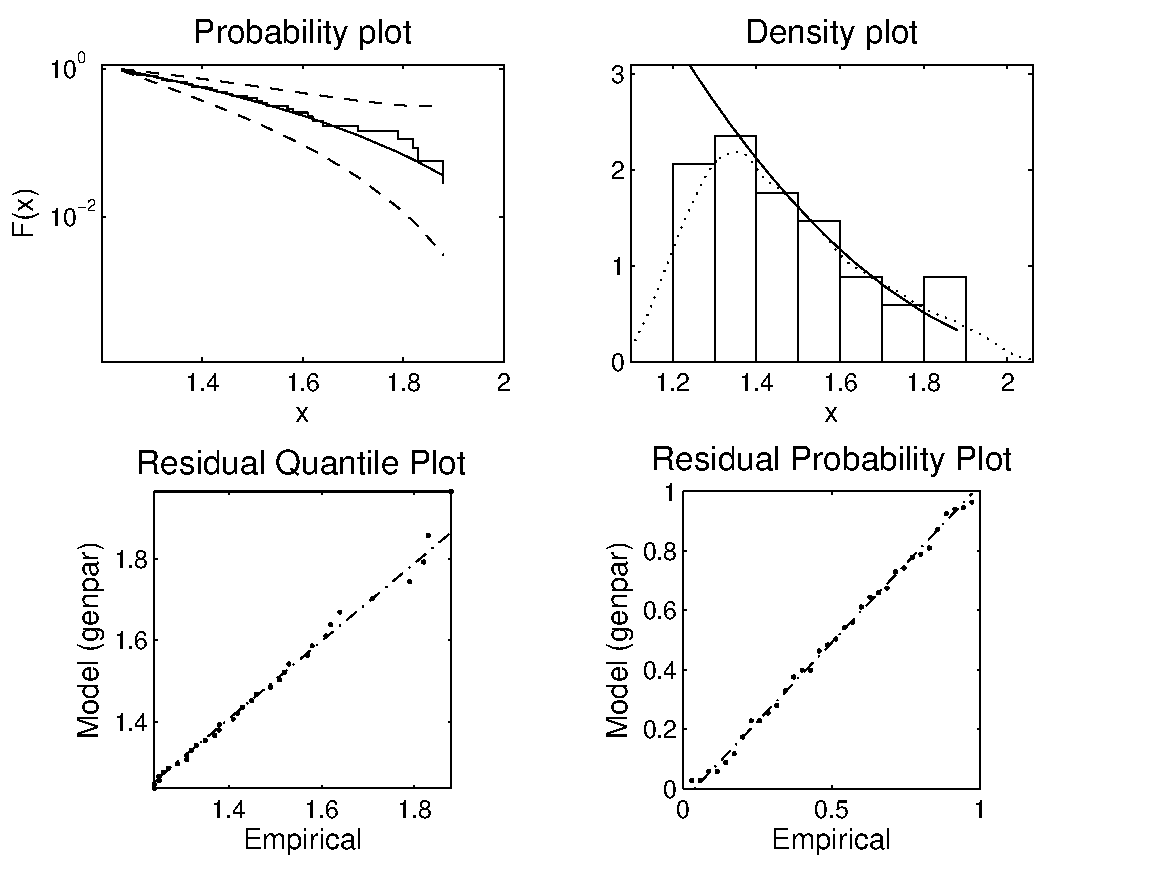
\includegraphics[width=\onefigwidth]{fig_decluster3b}}
\vspace{-3mm}
\caption[Diagnostic POT plot for sea data]{Diagnostic GPD plot for sea
data return levels.}
\label{fig:decluster3}
\end{figure}

\index[xentr]{Peaks Over Threshold analysis, POT|)}

\clearpage
\section{Summary of statistical procedures in \progname{}}
\label{sec:extremevaluestatistics}

The extreme value analysis presented in this chapter is part of a
comprehensive library of statistical routines for
random number generation, probability distributions, and parameter and density
estimation and likelihood analysis, etc.
{\small\begin{verbatim}
help statistics

  Module STATISTICS in WAFO Toolbox.
  Version 2.5.2  07-Feb-2011

  What's new
    Readme           - New features, bug fixes, and changes
                        in STATISTICS.

  Parameter estimation
    fitbeta          - Parameter estimates for Beta data
    fitchi2          - Parameter estimates for
                                 Chi squared data
    fitexp           - Parameter estimates for
                                 Exponential data
    fitgam           - Parameter estimates for Gamma data
    fitgengam        - Parameter estimates for
                                 Generalized Gamma data
    fitgenpar        - Parameter estimates for
                                 Generalized Pareto data
    fitgenparml      - Internal routine for fitgenpar
                       (ML estimates for GPD data)
    fitgenparrange   - Parameter estimates for GPD model
                                 over a range of thresholds
    fitgev           - Parameter estimates for GEV data
    fitgumb          - Parameter estimates for Gumbel data
    fitinvnorm       - Parameter estimates for
                                 Inverse Gaussian data
    fitlognorm       - Parameter estimates for Lognormal data
    fitmarg2d        - Parameter estimates for MARG2D data
    fitmargcnd2d     - Parameter estimates for DIST2D data
    fitnorm          - Parameter estimates for Normal data
    fitray           - Parameter estimates for Rayleigh data
    fitraymod        - Parameter estimates for
                                 Truncated Rayleigh data
    fitt             - Parameter estimates for
                                 Student's T data
    fitweib          - Parameter estimates for Weibull data
    fitweib2d        - Parameter estimates for 2D Weibull data
    fitweibmod       - Parameter estimates for
                                 truncated Weibull data

    likgenpar        - Log likelihood function for GPD
    likweib2d        - 2D Weibull log-likelihood function

    loglike          - Negative Log-likelihood function.
    logps            - Moran's negative log Product
                                 Spacings statistic
    mlest            - Maximum Likelihood or Maximum Product
                       Spacing estimator

  Probability density functions (pdf)
    pdfbeta          - Beta PDF
    pdfbin           - Binomial PDF
    pdfcauchy        - Cauchy's PDF
    pdfchi2          - Chi squared PDF
    pdfdiscrete      - Discrete PDF
    pdfempirical     - Empirical PDF
    pdfexp           - Exponential PDF
    pdff             - Snedecor's F PDF
    pdffrech         - Frechet PDF
    pdfgam           - Gamma PDF
    pdfgengam        - Generalized Gamma PDF
    pdfgengammod     - Modified Generalized Gamma PDF (stable)
    pdfgenpar        - Generalized Pareto PDF
    pdfgev           - Generalized Extreme Value PDF
    pdfgumb          - Gumbel PDF.
    pdfhyge          - Hypergeometric probability mass function
    pdfinvnorm       - Inverse Gaussian PDF
    pdflognorm       - Lognormal PDF
    pdfmarg2d        - Joint 2D PDF due to Plackett given as
                       f{x1}*f{x2}*G(x1,x2;Psi).
    pdfmargcnd2d     - Joint 2D PDF computed as
                       f(x1|X2=x2)*f(x2)
    pdfnorm          - Normal PDF
    pdfnorm2d        - Bivariate Gaussian distribution
    pdfnormnd        - Multivariate Normal PDF
    pdfray           - Rayleigh PDF
    pdfraymod        - Truncated Rayleigh PDF
    pdft             - Student's T PDF
    pdfpois          - Poisson probability mass function
    pdfweib          - Weibull PDF
    pdfweib2d        - 2D Weibull PDF
    pdfweibmod       - Truncated Weibull PDF

  Cumulative distribution functions (cdf)
    cdfcauchy        - Cauchy CDF
    cdfdiscrete      - Discrete CDF
    cdfempirical     - Empirical CDF
    cdfmarg2d        - Joint 2D CDF due to Plackett
    cdfmargcnd2d     - Joint 2D CDF computed as
                       int F(X1<v|X2=x2).*f(x2)dx2
    cdfmargcnd2dfun  - is an internal function to cdfmargcnd2d
                       and prbmargcnd2d.
    cdfnormnd        - Multivariate normal CDF
    cdfweib2d        - Joint 2D Weibull CDF
    cdfbeta          - Beta CDF
    cdfbin           - Binomial CDF
    cdfchi2          - Chi squared CDF
    cdfexp           - Exponential CDF
    cdff             - Snedecor's F CDF
    cdffrech         - Frechet CDF
    cdfgam           - Gamma CDF
    cdfgengam        - Generalized Gamma CDF
    cdfgengammod     - Modified Generalized Gamma CDF
    cdfgenpar        - Generalized Pareto CDF
    cdfgev           - Generalized Extreme Value CDF
    cdfgumb          - Gumbel CDF
    cdfhyge          - The hypergeometric CDF
    cdfinvnorm       - Inverse Gaussian CDF
    cdflognorm       - Lognormal CDF
    cdfmargcnd2d     - Joint 2D CDF computed as
                       int F(X1<v|X2=x2).*f(x2)dx2
    cdfnorm          - Normal CDF
    cdfray           - Rayleigh CDF
    cdfraymod        - Modified Rayleigh CDF
    cdft             - Student's T CDF
    cdfpois          - Poisson CDF
    cdfweib          - Weibull CDF
    cdfweibmod       - Truncated Weibull CDF

    edf              - Empirical Distribution Function
    edfcnd           - Empirical Distribution Function
                       conditioned on X>=c

    prbmargcnd2d     - returns the probability for rectangular
                       regions
    prbweib2d        - returns the probability for rectangular
                       regions
    margcnd2dsmfun   - Smooths the MARGCND2D distribution
                       parameters
    margcnd2dsmfun2  - Smooths the MARGCND2D distribution
                       parameters

  Inverse cumulative distribution functions
    invbeta          - Inverse of the Beta CDF
    invbin           - Inverse of the Binomial CDF
    invcauchy        - Inverse of the Cauchy CDF
    invchi2          - Inverse of the Chi squared CDF
    invcmarg2d       - Inverse of the conditional CDF of
                       X2 given X1
    invcweib2d       - Inverse of the conditional 2D weibull
                       CDF of X2 given X1
    invdiscrete      - Disrete quantile
    invempirical     - Empirical quantile
    invexp           - Inverse of the Exponential CDF
    invf             - Inverse of Snedecor's F CDF
    invfrech         - Inverse of the Frechet CDF
    invgam           - Inverse of the Gamma CDF
    invgengam        - Inverse of the Generalized Gamma CDF
    invgengammod     - Inverse of the Generalized Gamma CDF
    invgenpar        - Inverse of the Generalized Pareto CDF
    invgev           - Inverse of the Generalized
                       Extreme Value CDF
    invgumb          - Inverse of the Gumbel CDF
    invhyge          - Inverse of the Hypergeometric CDF
    invinvnorm       - Inverse of the Inverse Ga(ussian CDF
    invlognorm       - Inverse of the Lognormal CDF
    invnorm          - Inverse of the Normal CDF
    invray           - Inverse of the Rayleigh CDF
    invt             - Inverse of the Student's T CDF
    invweib          - Inverse of the Weibull CDF
    invpois          - Inverse of the Poisson CDF
    invraymod        - Inverse of the modified Rayleigh CDF
    invweibmod       - Inverse of the modified Weibull CDF

  Random number generators
    rndalpha         - Random matrices from a symmetric
                       alpha-stable distribution
    rndbeta          - Random matrices from a Beta distribution
    rndbin           - Random numbers from the binomial
                       distribution
    rndboot          - Simulate a bootstrap resample from a
                       sample
    rndcauchy        - Random matrices a the Cauchy
                       distribution
    rndchi2          - Random matrices from a Chi squared
                       distribution
    rnddiscrete      - Random sample
    rndempirical     - Bootstrap sample
    rndexp           - Random matrices from an Exponential
                       distribution
    rndf             - Random matrices from Snedecor's F
                       distribution
    rndfrech         - Random matrices from a Frechet
                       distribution
    rndgam           - Random matrices from a Gamma distribution
    rndgengam        - Random matrices from a Generalized Gamma
                       distribution.
    rndgengammod     - Random matrices from a Generalized
                       Modified Gamma distribution.
    rndgenpar        - Random matrices from a Generalized Pareto
                       Distribution
    rndgev           - Random matrices from a Generalized
                       Extreme Value distribution
    rndgumb          - Random matrices from a Gumbel
                       distribution
    rndhyge          - Random numbers from the Hypergeometric
                       distribution
    rndinvnorm       - Random matrices from a Inverse Gaussian
                       distribution
    rndlognorm       - Random matrices from a Lognormal
                       distribution.
    rndmarg2d        - Random points from a MARG2D
                       distribution
    rndmargcnd2d     - Random points from a MARGCND2D
                       distribution
    rndnorm          - Random matrices from a Normal
                       distribution
    rndnormnd        - Random vectors from a multivariate
                       Normal distribution
    rndpois          - Random matrices from a Poisson
                       distribution
    rndray           - Random matrices from a Rayleigh
                       distribution
    rndraymod        - Random matrices from modified Rayleigh
                       distribution
    rndt             - Random matrices from a Student's T
                       distribution
    rndweib          - Random matrices a the Weibull
                       distribution
    rndweibmod       - Random matrices from the modified Weibull
                       distribution
    rndweib2d        - Random numbers from the 2D Weibull
                       distribution

  Moments
    mombeta          - Mean and variance for the Beta
                       distribution
    mombin           - Mean and variance for the Binomial
                       distribution
    momchi2          - Mean and variance for the Chi squared
                       distribution
    momexp           - Mean and variance for the Exponential
                       distribution
    momf             - Mean and variance for Snedecor's F
                       distribution
    momfrech         - Mean and variance for the Frechet
                       distribution
    momgam           - Mean and variance for the Gamma
                       distribution
    momgengam        - Mean and variance for the Generalized
                       Gamma distribution
    momgenpar        - Mean and variance for the Generalized
                       Pareto distribution
    momgev           - Mean and variance for the GEV
                       distribution
    momgumb          - Mean and variance for the Gumbel
                       distribution
    momhyge          - Mean and variance for the Hypergeometric
                       distribution
    mominvnorm       - Mean and variance for the Inverse
                       Gaussian distribution
    momlognorm       - Mean and variance for the Lognormal
                       distribution
    mommarg2d        - Mean and variance for the MARG2D
                       distribution
    mommargcnd2d     - Mean and variance for the MARGCND2D
                       distribution
    momnorm          - Mean and variance for the Normal
                       distribution
    mompois          - Mean and variance for the Poisson
                       distribution
    momray           - Mean and variance for the Rayleigh
                       distribution
    momt             - Mean and variance for the Student's T
                       distribution
    momweib          - Mean and variance for the Weibull
                       distribution
    momweib2d        - Mean and variance for the 2D Weibull
                       distribution

  Profile log likelihood functions
    lnkexp           - Link for x,F and parameters of
                       Exponential distribution
    lnkgenpar        - Link for x,F and parameters of
                       Generalized Pareto distribution
    lnkgev           - Link for x,F and parameters of
                       Generalized Extreme value distribution
    lnkgumb          - Link for x,F and parameters of Gumbel
                       distribution
    lnkgumbtrnc      - Link for x,F and parameters of truncated
                       Gumbel distribution
    lnkray           - Link for x,F and parameters of Rayleigh
                       distribution
    lnkweib          - Link for x,F and parameters of Weibull
                       distribution
    loglike          - Negative Log-likelihood function
    logps            - Moran's negative log Product Spacings
                       statistic
    ciproflog        - Confidence Interval using Profile Log-
                       likelihood or Product Spacing- function
    proflog          - Profile Log- likelihood or
                       Product Spacing-function
    findciproflog    - Find Confidence Interval from proflog
                       function

  Extremes
    decluster        - Decluster peaks over threshold values
    extremalidx      - Extremal Index measuring the dependence
                       of data
    findpot          - Find indices to Peaks over threshold
                       values
    fitgev           - Parameter estimates for GEV data
    fitgenpar        - Parameter estimates for Generalized
                       Pareto data
    prb2retper       - Return period from Probability of
                       exceedance
    retper2prb       - Probability of exceedance from return
                       period

  Threshold selection
    fitgenparrange   - Parameter estimates for GPD model vs
                       thresholds
    disprsnidx       - Dispersion Index vs threshold
    reslife          - Mean Residual Life, i.e., mean excesses
                       vs thresholds
    plotdisprsnidx   - Plot Dispersion Index vs thresholds
    plotreslife      - Plot Mean Residual Life
                       (mean excess vs thresholds)

  Regression models
    logit            - Logit function.
    logitinv         - Inverse logit function.
    regglm           - Generalized Linear Model regression
    reglm            - Fit multiple Linear Regression Model.
    reglogit         - Fit ordinal logistic regression model.
    regnonlm         - Non-Linear Model Regression
    regsteplm        - Stepwise predictor subset selection for
                       Linear Model regression

  Factor analysis
    princomp         -  Compute principal components of X

  Descriptive Statistics
    ranktrf          - Rank transformation of data material.
    spearman         - Spearman's rank correlation coefficient
    mean             - Computes sample mean (Matlab)
    median           - Computes sample median value (Matlab)
    std              - Computes standard deviation (Matlab)
    var              - Computes sample variance (Matlab)
    var2corr         - Variance matrix to correlation matrix
                       conversion
    cov              - Computes sample covariance matrix
                       (Matlab)
    corrcoef         - Computes sample correlation coefficients
                       (Matlab toolbox)
    skew             - Computes sample skewness
    kurt             - Computes sample kurtosis
    lmoment          - L-moment based on order statistics
    percentile       - Empirical quantile (percentile)
    iqrange          - Computes the Inter Quartile Range
    range            - Computes the range between the maximum
                       and minimum values

  Statistical plotting
    clickslct        - Select points in a plot by clicking
                       with the mouse
    histgrm          - Plot histogram
    plotbox          - Plot box-and-whisker diagram
    plotdensity      - Plot density.
    plotexp          - Plot data on Exponential distribution
                       paper
    plotedf          - Plot Empirical Distribution Function
    plotedfcnd       - Plot Empirical Distribution Function
                       CoNDitioned that X>=c
    plotfitsumry     - Plot diagnostic of fit to data
    plotgumb         - Plot data on Gumbel distribution paper
    plotkde          - Plot kernel density estimate of PDF
    plotmarg2dcdf    - Plot conditional CDF of X1 given X2=x2
    plotmarg2dmom    - Plot conditional mean and standard
                       deviation
    plotmargcnd2dcdf - Plot conditional empirical CDF of X1
                       given X2=x2
    plotmargcnd2dfit - Plot parameters of the conditional
                       distribution
    plotmargcnd2dmom - Plot conditional mean and
                       standard deviation
    plotnorm         - Plot data on a Normal distribution paper
    plotqq           - Plot empirical quantile of X vs empirical
                       quantile of Y
    plotray          - Plot data on a Rayleigh distribution
                       paper
    plotresprb       - Plot Residual Probability
    plotresq         - Plot Residual Quantile
    plotscatr        - Pairwise scatter plots
    plotweib         - Plot data on a Weibull distribution paper
    plotweib2dcdf    - Plot conditional empirical CDF of X1
                       given X2=x2
    plotweib2dmom    - Plot conditional mean and standard
                       deviation

  Hypothesis Tests
    anovan           - multi-way analysis of variance (ANOVA)
    testgumb         - Tests if shape parameter in a GEV is
                       equal to zero
    testmean1boot    - Bootstrap t-test for the mean equal to 0
    testmean1n       - Test for mean equals 0 using
                       one-sample T-test
    testmean2n       - Two-sample t-test for mean(x) equals
                       mean(y)
    testmean1r       - Wilcoxon signed rank test for
                       H0: mean(x) equals 0
    testmean2r       - Wilcoxon rank-sum test for
                       H0: mean(x) equals mean(y)

  Confidence interval estimation
    ciboot           - Bootstrap confidence interval.
    ciquant          - Nonparametric confidence interval for quantile
    momci1b          - Moment confidence intervals using
                       Bootstrap

  Bootstrap & jacknife estimates
    covboot          - Bootstrap estimate of the variance of
                       a parameter estimate.
    covjack          - Jackknife estimate of the variance of
                       a parameter estimate.
    stdboot          - Bootstrap estimate of the
                       standard deviation of a parameter
    stdjack          - Jackknife estimate of the
                       standard deviation of a parameter

  Design of Experiments
    yates            - Calculates main and interaction effects
                       using Yates' algorithm.
    ryates           - Reverse Yates' algorithm to give
                       estimated responses
    fitmodel         - Fits response by polynomial
    alias            - Alias structure of a fractional design
    cdr              - Complete Defining Relation
    cl2cnr           - Column Label to Column Number
    cnr2cl           - Column Number to Column Label
    ffd              - Two-level Fractional Factorial Design
    getmodel         - Return the model parameters
    sudg             - Some Useful Design Generators
    plotresponse     - Cubic plot of responses
    nplot            - Normal probability plot of effects

  Misc
    comnsize         - Calculates common size of all non-scalar
                       arguments
    dgammainc        - Incomplete gamma function with derivatives
    gammaincln       - Logarithm of incomplete gamma function.
    parsestatsinput  - Parses inputs to pdfxx, prbxx, invxx and
                       rndxx functions
    createfdata      - Distribution parameter struct constructor
    getdistname      - Return the distribution name

    stdize           - Standardize columns to have mean 0 and
                       standard deviation 1
    center           - Recenter columns to have mean 0

   Demo
    demofitgenpar    - Script to check the variance of estimated
                       parameters
\end{verbatim}
    }


%\bibliography{wafoBibliography}

%%% Local Variables:
%%% mode: latex
%%% TeX-master: "wafomanual"
%%% End:
